\chapter{Sistema multisensorial }
\label{cap:capitulo4}

%\begin{flushright}
%\begin{minipage}[]{10cm}
%\emph{Quizás algún fragmento de libro inspirador...}\\
%\end{minipage}\\

%Autor, \textit{Título}\\
%\end{flushright}

\vspace{1cm}
Este capítulo consta de la descripción detallada del proceso que se ha llevado a cabo para crear el sistema multisensorial para la monitorización de animales de laboratorio. Como se ha introducido previamente, la base idea de este trabajo ha sido pensada para un laboratorio de animales. Debido al desconocimiento de robótica de los trabajadores de este sector, puede haber trabajo que se realice en el laboratorio que podría mejorarse e incluso automatizarse.\\

Para obtener más información, se ha contactado con el Laboratorio del Bienestar e Investigación Animal de la Universidad de Alcalá de Henares \footnote{\url{https://www.uah.es/es/investigacion/unidades-de-investigacion/grupos-de-investigacion/Bienestar-en-Investigacion-Animal-Welfare-on-Animal-Research./}} para conocer la situación en la que trabajan. Se han apreciado bastantes cosas mejorables y se ha enfocado el objetivo en la monitorización de los ratones del laboratorio, que requieren una observación constante así como del entorno en el que se encuentran debido a que deben estar bajo unas condiciones determinadas.\\

Asimismo, para facilitar la comprensión de los datos, se ofrece una interfaz gráfica donde los valores numéricos obtenidos por los sensores, así como cualquier interacción necesaria en la IU se traducen en \textit{widgets} ---pequeñas imágenes que proveen información visual--- comprensibles para cualquier usuario de una manera intuitiva y sencilla.\\

Dos son las partes esenciales para el desarrollo: hardware y software. En la primera sección se presenta el desarrollo hardware y en la sección posterior el desarrollo software que se ha realizado para tener un funcionamiento correcto del sistema.

\section{Desarrollo hardware}
La placa que se ha utilizado para el proyecto es la Raspberry Pi 4B (Figura \ref{fig:rasp}), el último modelo de Raspberry y muy utilizada para el desarrollo de proyectos debido a su bajo coste. Este modelo es el más rápido y potente, ofreciendo de dos a tres veces el rendimiento del procesador de su modelo predecesor. El sistema operativo utilizado para el desarrollo del proyecto ha sido Raspbian.\\
\begin{figure} [h!]
  \begin{center}
    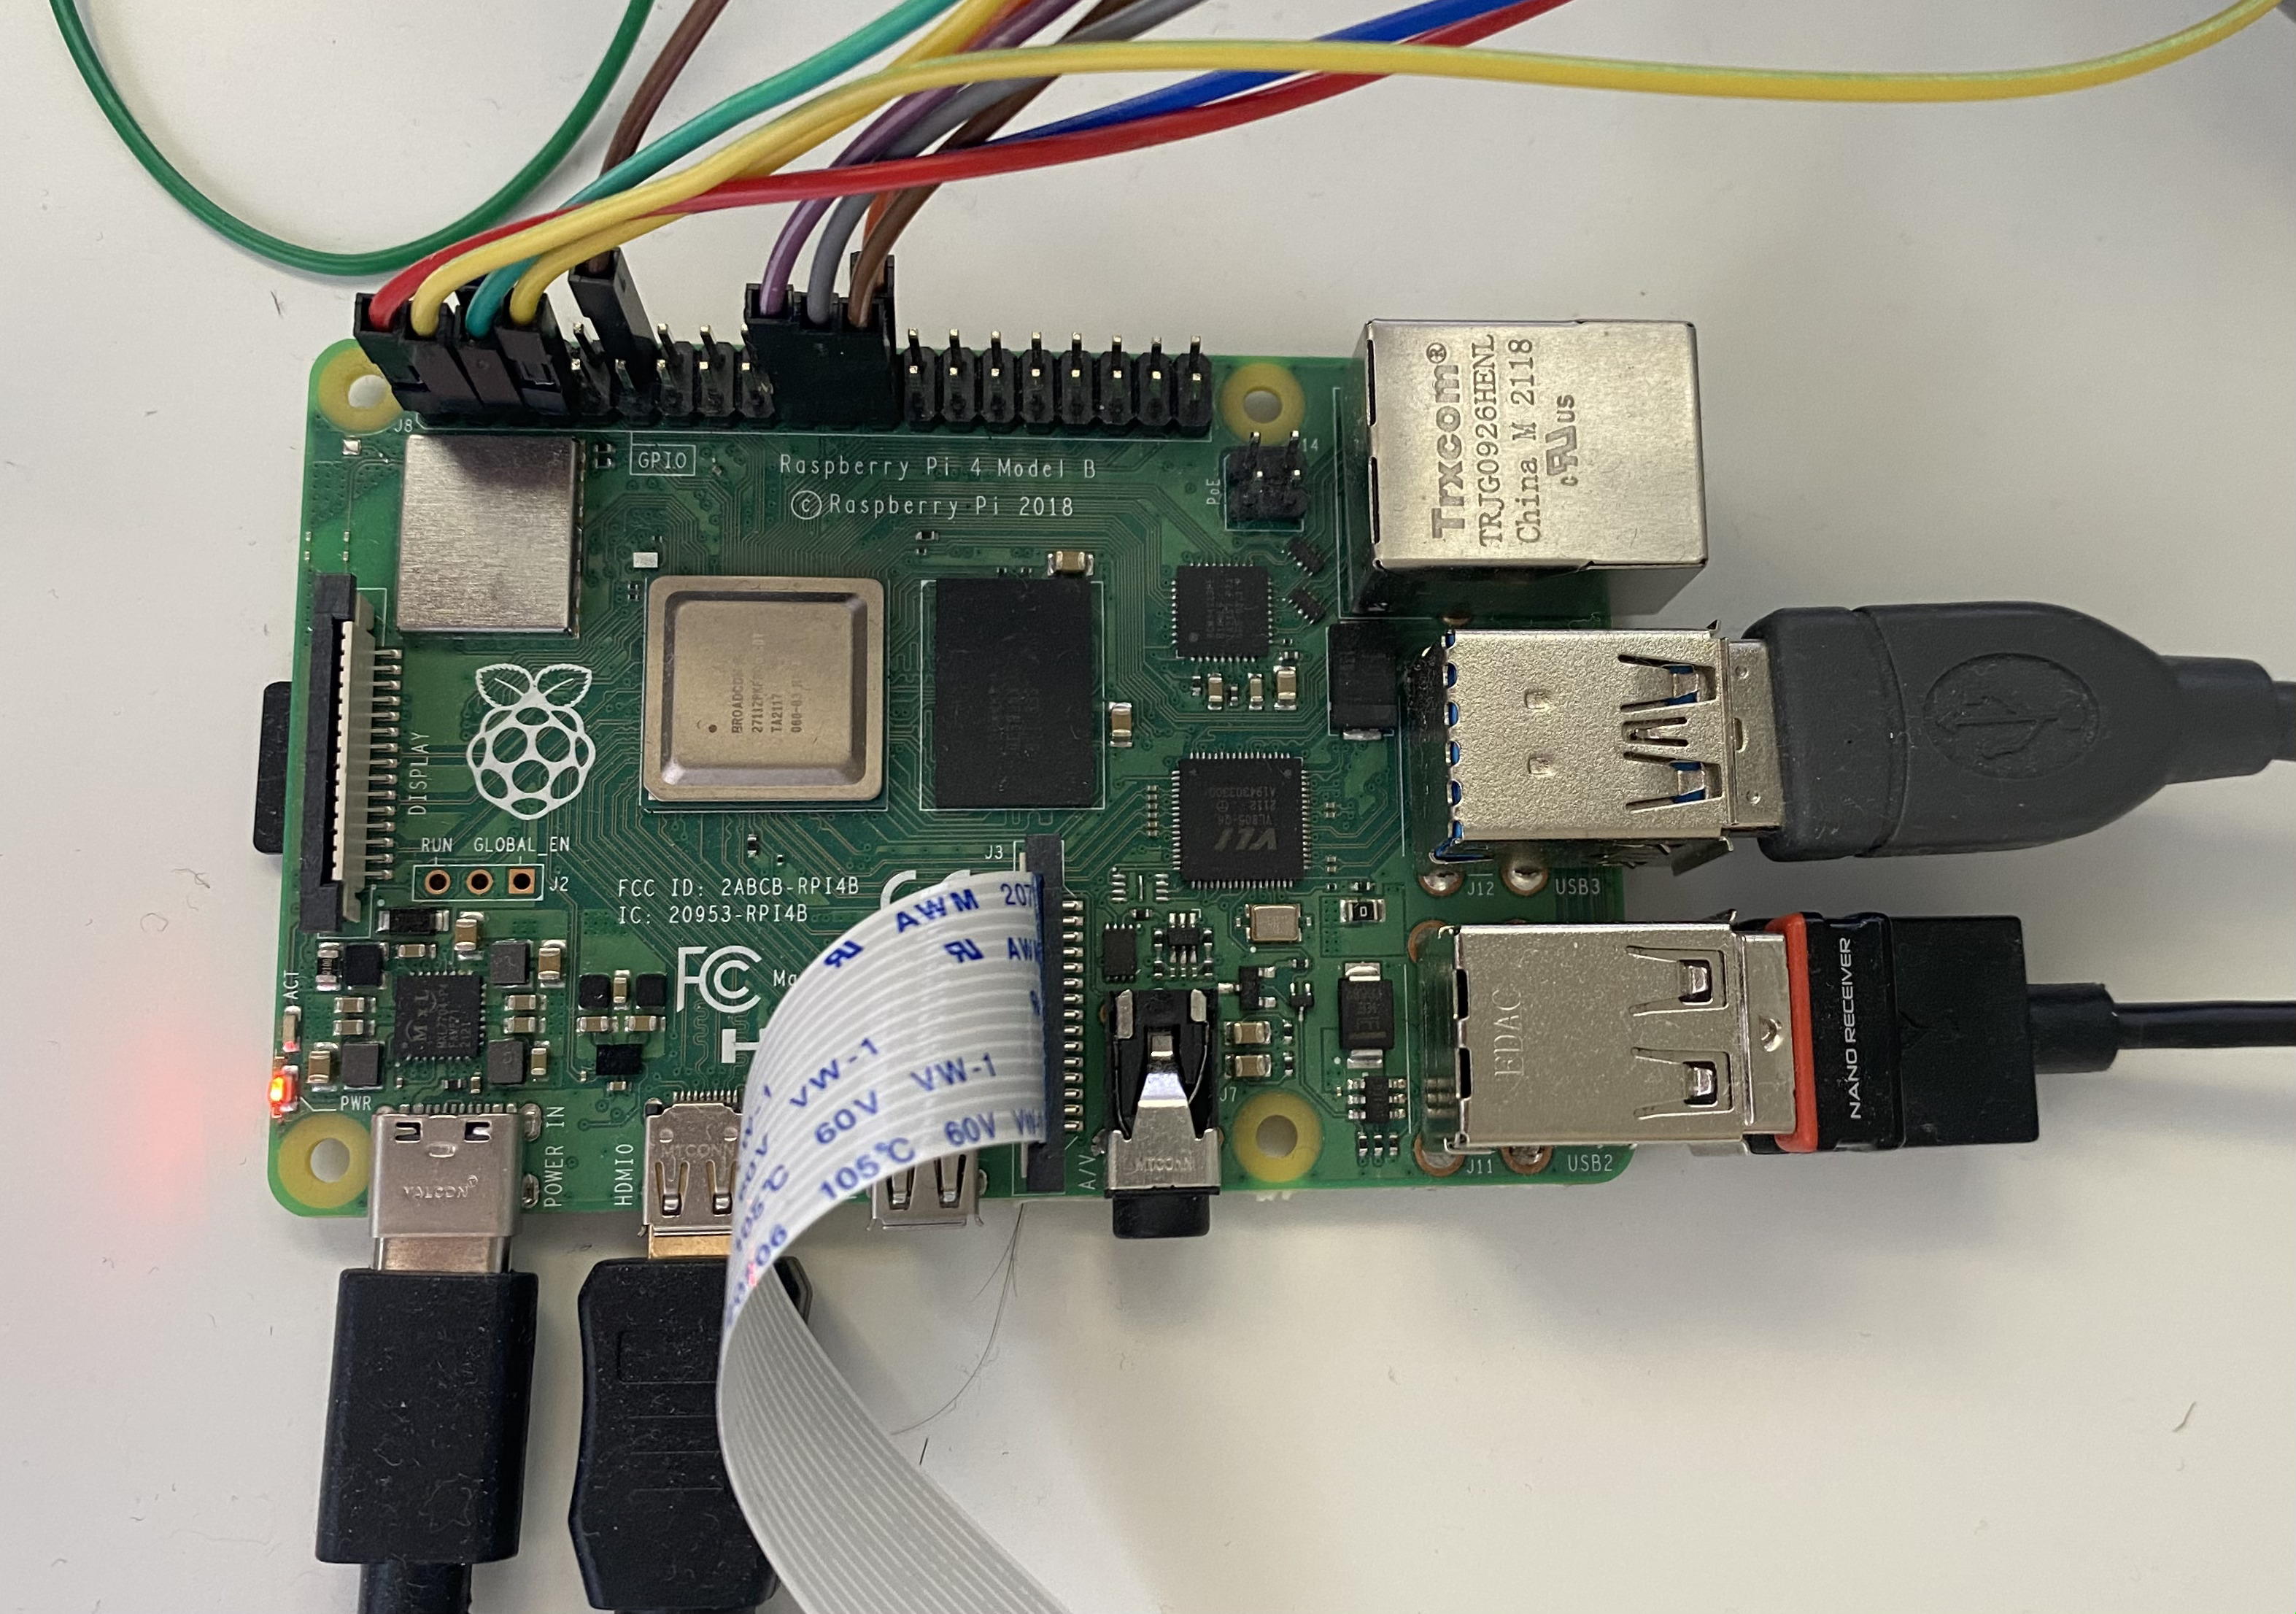
\includegraphics[width=8cm]{figs/raspberry}
  \end{center}
  \caption{Raspberry Pi 4B utilizada para el desarrollo del presente TFG.}
  \label{fig:rasp}
\end{figure}

Está dotada de una serie de pines y puertos que permiten su conexión con distintos sensores o actuadores. Para este trabajo se han utilizado los sensores presentados en el capítulo \ref{sec:hw}. A continuación se explican con más detalle estos sensores:
\begin{itemize}
\item{Sensor BME680 (Figura \ref{fig:bme_of}).} Este sensor es capaz de medir hasta cuatro parámetros: el gas, la temperatura, la presión y la humedad.

\item{Sensor AMG8833 (Figura \ref{fig:termicos}-a).} Este sensor es una cámara térmica que permite recibir la información del entorno y mostrarla a través de un rango de colores. Los colores más cálidos ---como el rojo--- indican la presencia de mayor temperatura, mientras que los colores fríos ---como el azul--- indican una temperatura inferior. Los valores que ofrece este sensor es una matriz de 8x8 valores de temperatura, que deben ser traducidos para poder visualizar la imagen de temperaturas (Figura \ref{fig:temps}).

\item{Sensor DS18B20 (Figura \ref{fig:ds_of}).} Este sensor permite medir la temperatura en superficies húmedas, ya que es resistente al agua.

\item{MQ-135 (Figura \ref{fig:mq_of}).} Este sensor permite medir la calidad de distintos gases, entre ellos el de amoníaco. Es muy importante tener controlada la cantidad de amoníaco en el entorno de los ratones. Este sensor también realiza lecturas analógicas, por lo que es necesario el uso de un conversor analógico a digital.

\item{Sensor nivel de agua (Figura \ref{fig:nivel_of}).} Con este sensor se puede medir la presencia de agua, así como la cantidad de agua que hay. Este sensor tiene lecturas analógicas, por lo que es necesario el uso de un conversor analógico a digital.

\item{Seek thermal (Figura \ref{fig:termicos}-b).} Este sensor es una cámara térmica. Permite obtener imágenes representando las temperaturas con colores de la misma forma que el sensor \ref{fig:termicos}-a, pero con mucha más calidad y precisión.

\item{PiCamera (Figura \ref{fig:picam_of}).} Este sensor es una de las cámaras oficiales de Raspberry, que permite obtener imágenes del entorno y mostrarlas en pantalla.
\end{itemize}

\begin{figure} [h!]
  \begin{center}
    \includegraphics[width=8cm]{figs/temps}
  \end{center}
  \caption{Imagen generada después de la conversión de los datos numéricos.}
  \label{fig:temps}
\end{figure}

Raspberry no tiene lecturas analógicas, por lo que ha sido necesario el uso de un conversor analógico a digital (el MCP3008) para la lectura del sensor MQ-135 \ref{fig:mq_of} y el sensor de nivel de agua \ref{fig:nivel_of}. Además, se han utilizado otros componentes como son resistencias o leds para el correcto funcionamiento de los sensores y proporcionar al usuario mayor comprensión del funcionamiento del sistema.\\

En la figura \ref{fig:esquema} se puede ver un esquema de los sensores utilizados integrados en la Raspberry.
\begin{figure} [h!]
  \begin{center}
    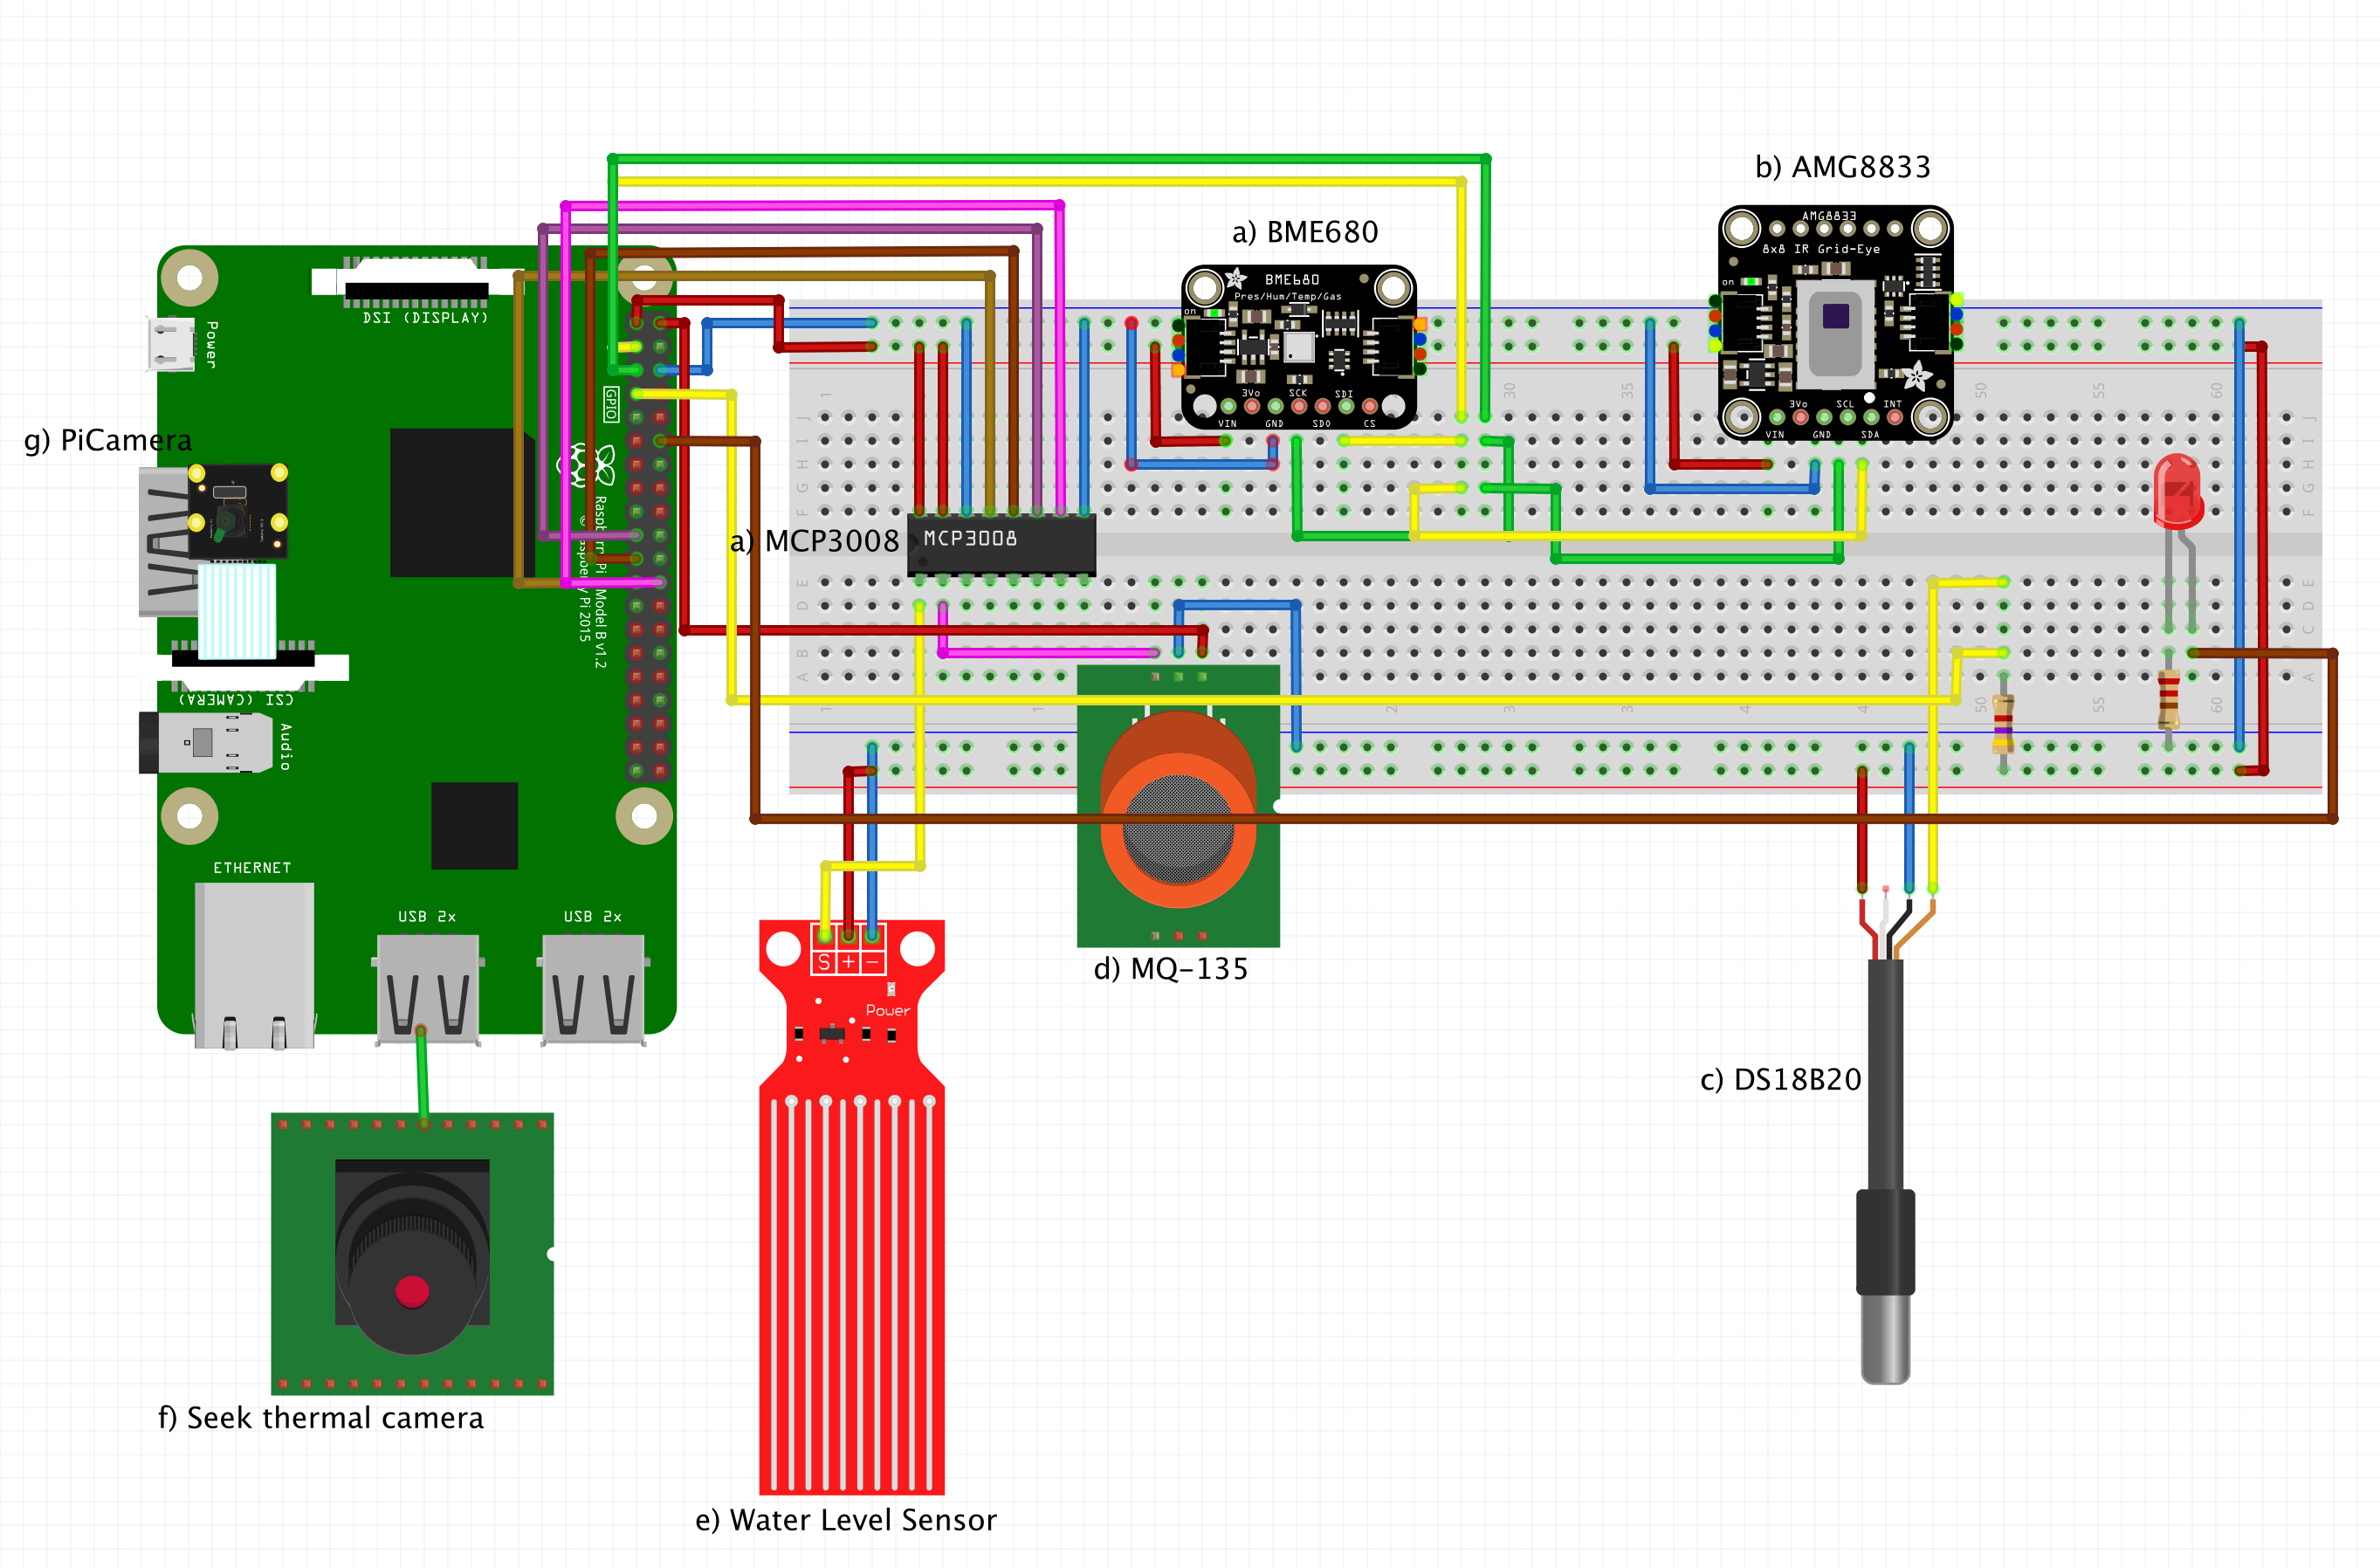
\includegraphics[width=14cm]{figs/esquema}
  \end{center}
  \caption{Esquema de conexiones.}
  \label{fig:esquema}
\end{figure}\\

\section{Desarrollo software}
Tras disponer de la parte hardware, el equipo está preparado. Para que este equipo funcione, es necesario crear las instrucciones y reglas a través de programas o aplicaciones, esto es, la parte software.\\

Como se ha comentado previamente, se han mantenido reuniones con el laboratorio así como reuniones semanales con el tutor. De estas reuniones se ha obtenido la información necesaria para realizar el proyecto. Además, ha permitido extraer el diagrama de casos de uso (Figura \ref{fig:casos}).\\
\begin{figure} [h!]
  \begin{center}
    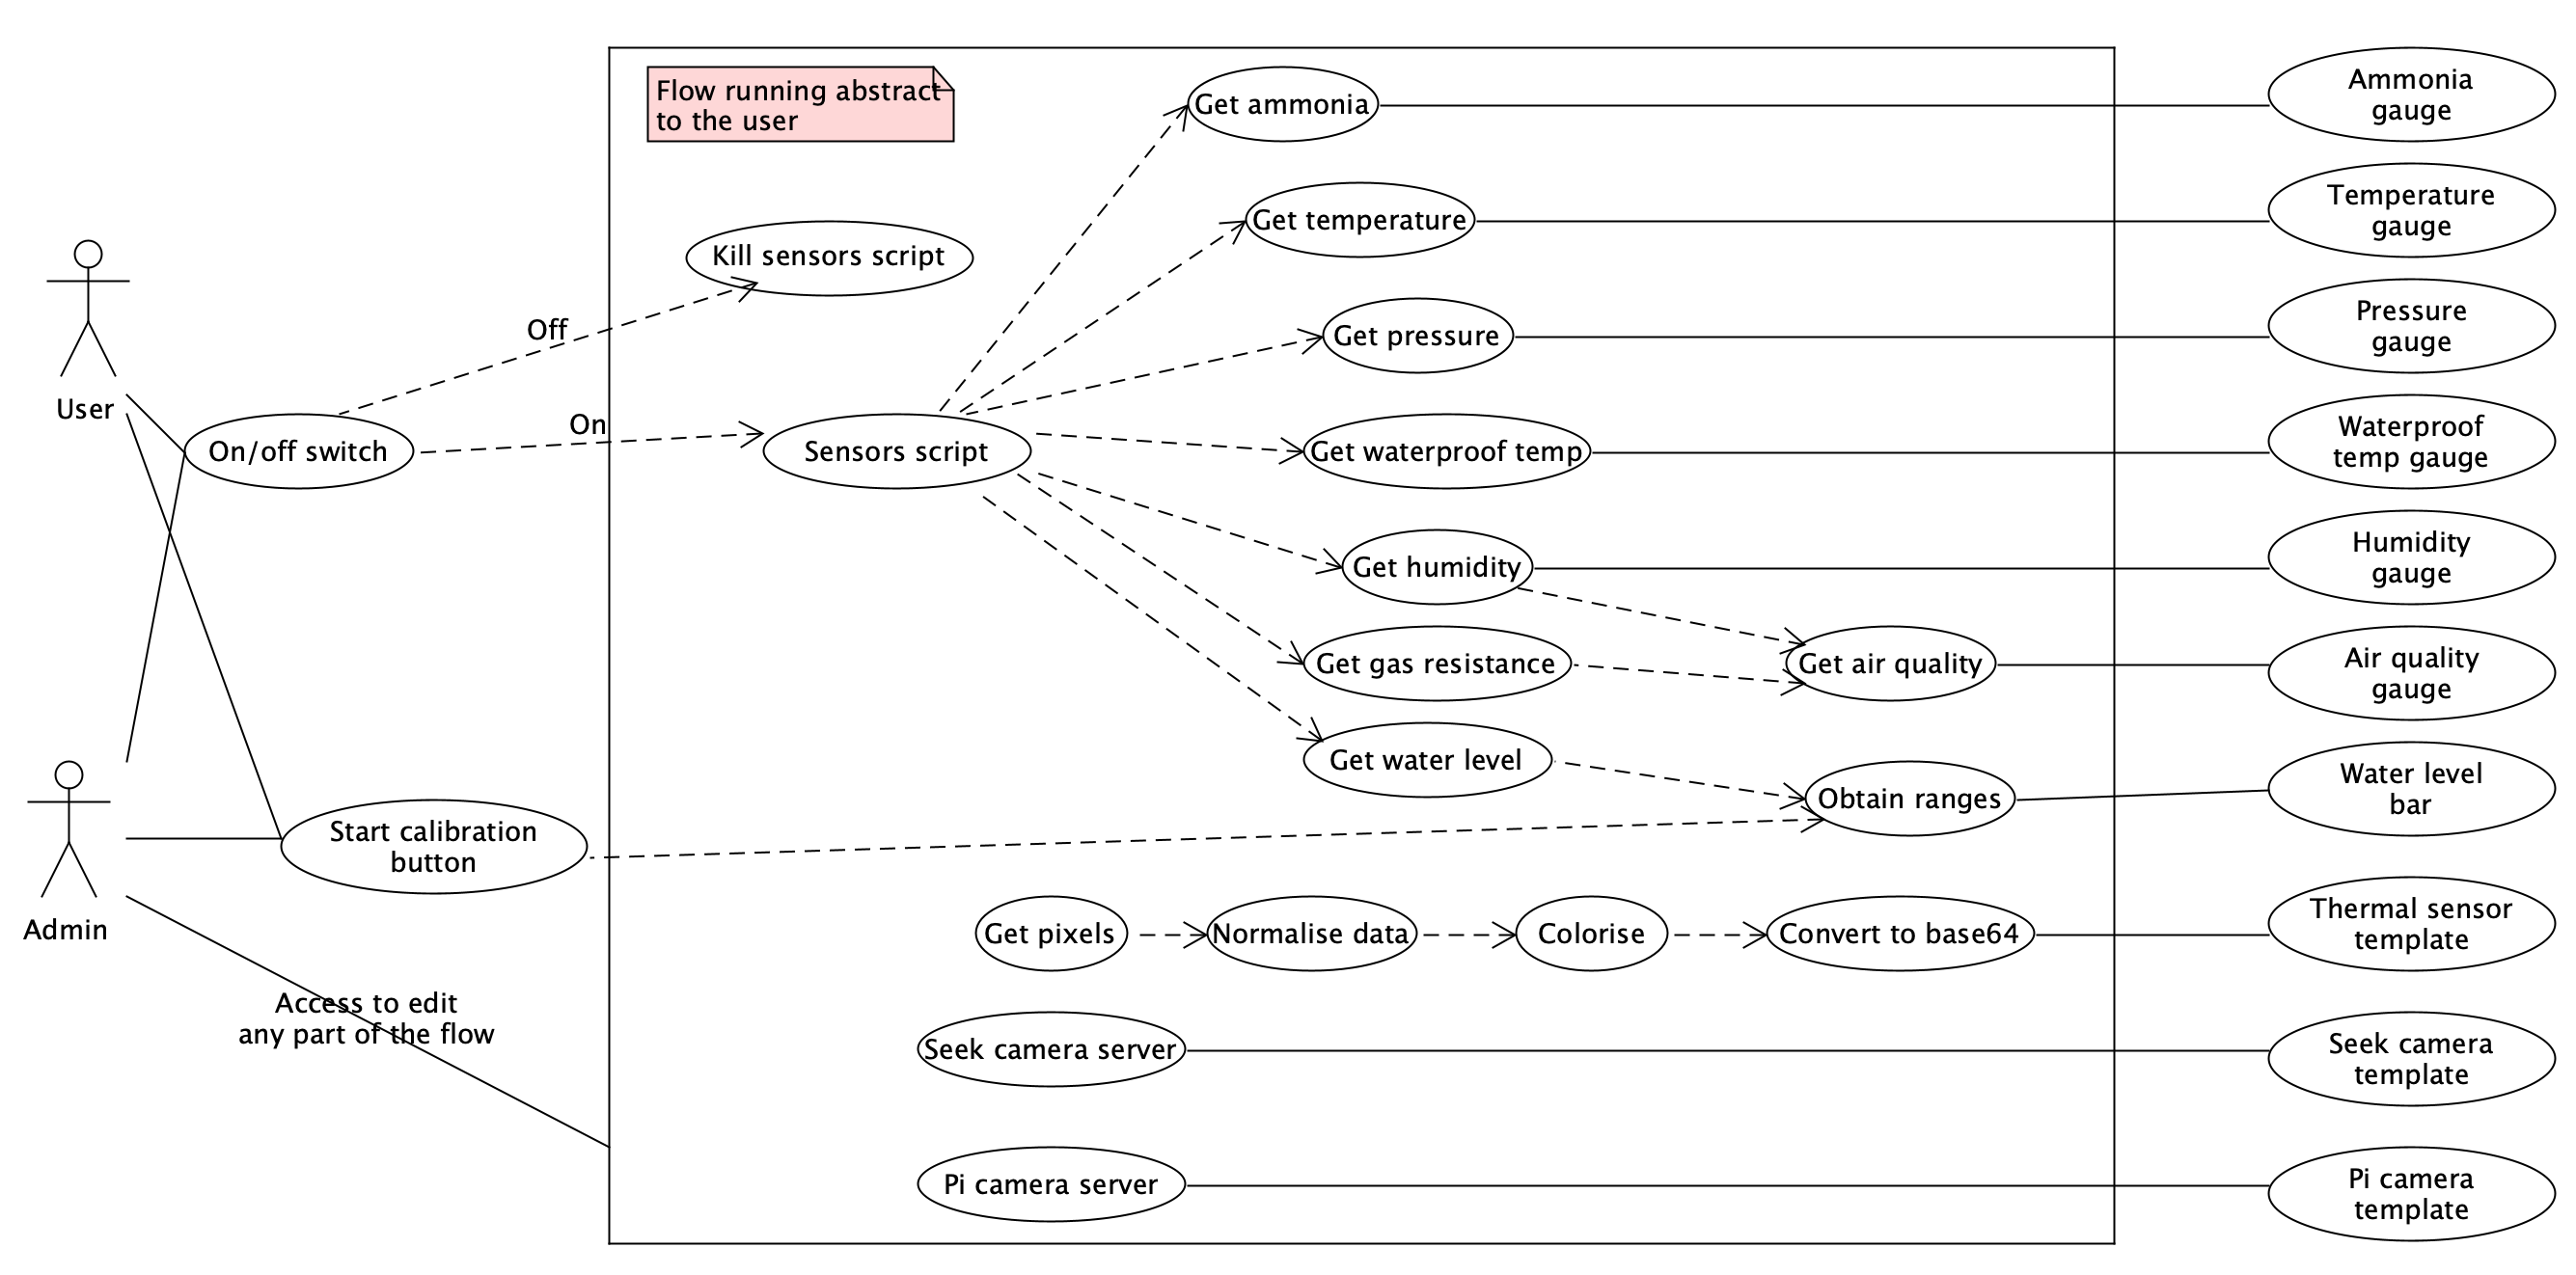
\includegraphics[width=17cm]{figs/casos}
  \end{center}
  \caption{Diagrama de casos de uso del proyecto.}
  \label{fig:casos}
\end{figure}

En base al diagrama de casos de uso, se debe crear un fichero que permita obtener todas las lecturas de los distintos sensores. Para proporcionar abstracción y mejorar el código, por cada sensor debe crearse una clase. Esto ha permitido crear el diagrama de clases visible en la Figura \ref{fig:umlet} para ser implementado.\\
\begin{figure} [h!]
  \begin{center}
    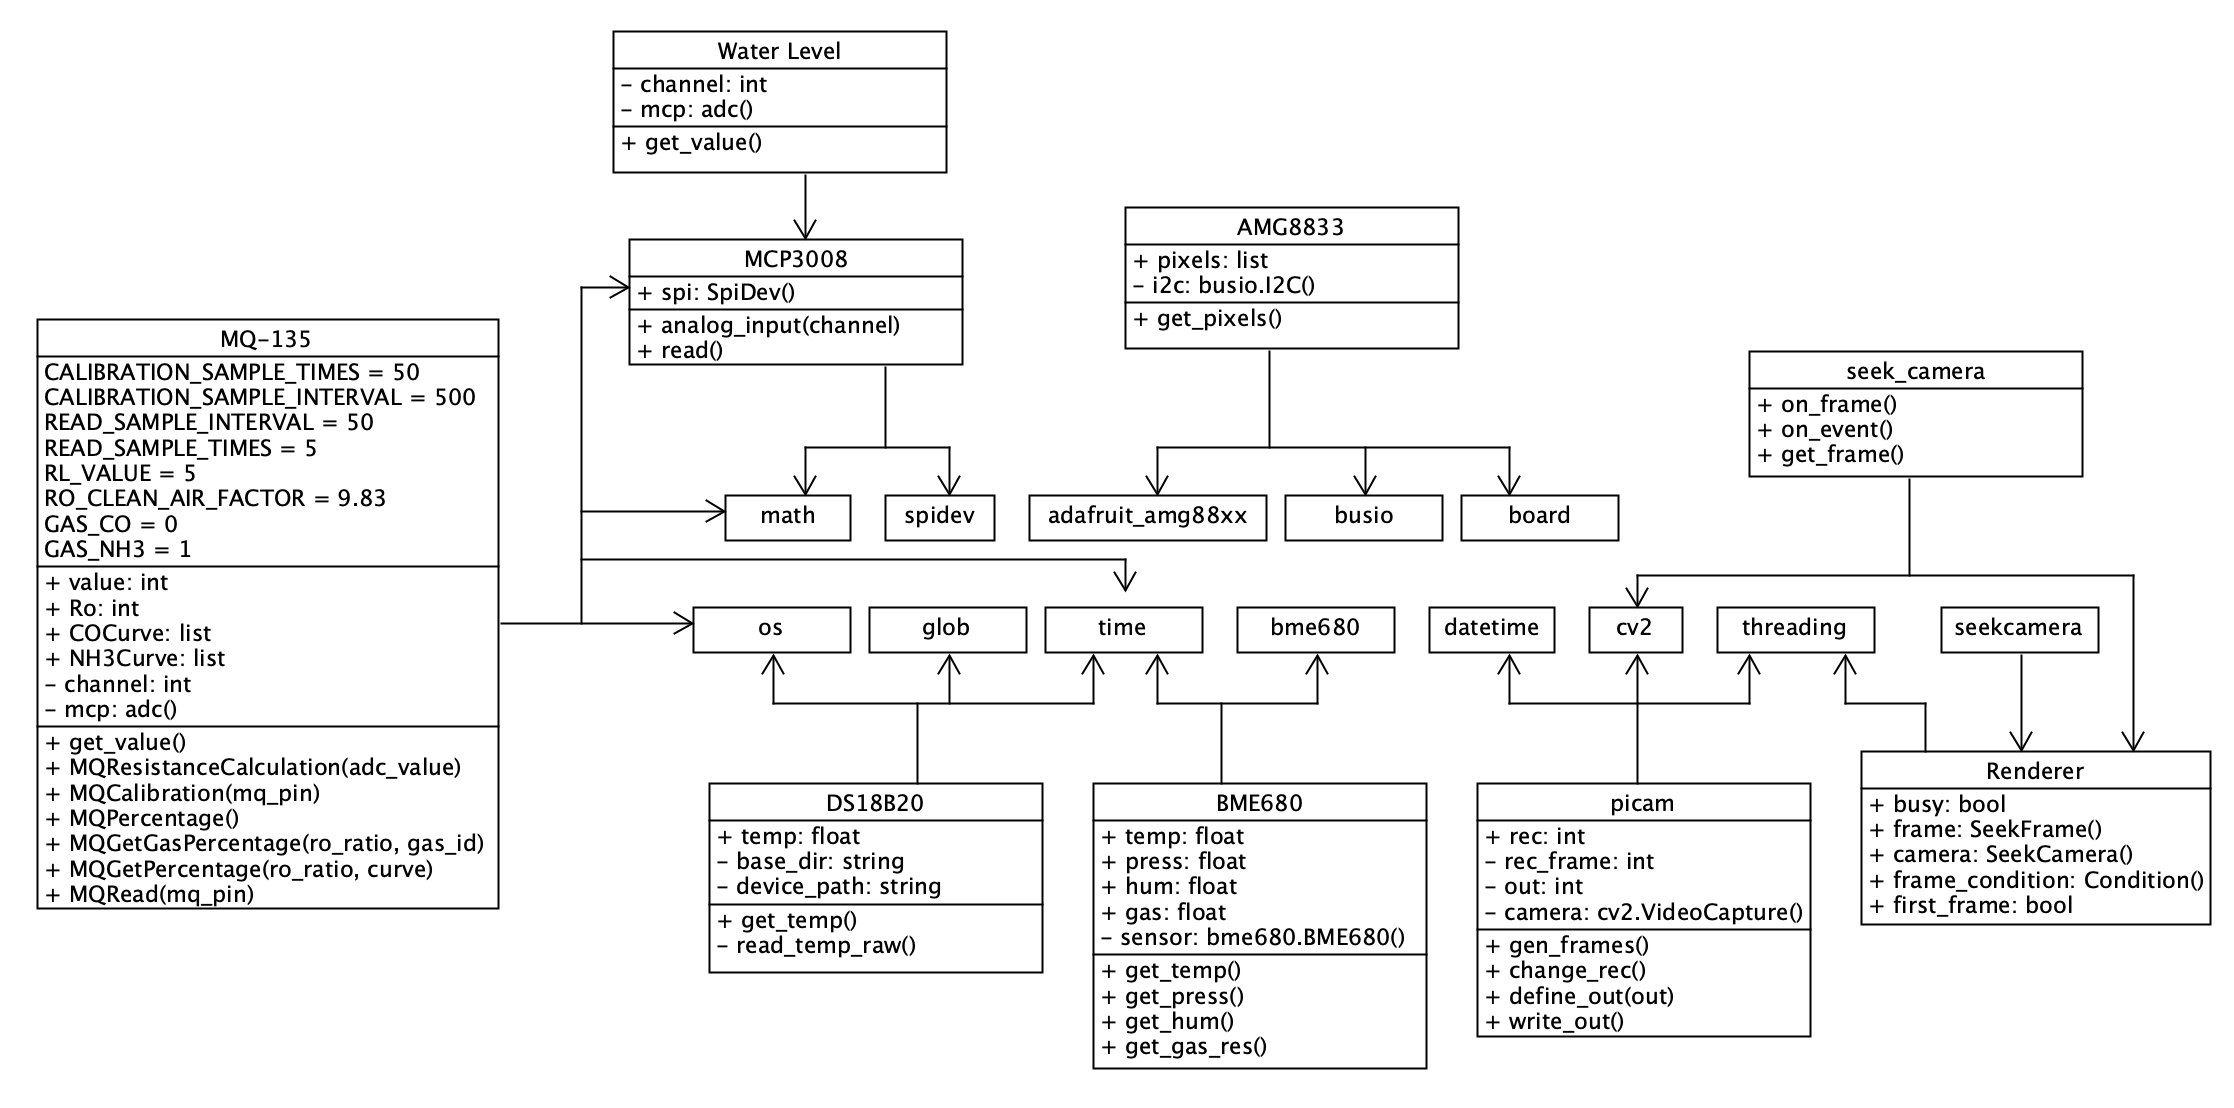
\includegraphics[width=14cm]{figs/umlet}
  \end{center}
  \caption{Esquema de clases de cada sensor hecho en UMLet.}
  \label{fig:umlet}
\end{figure}

En primer lugar ha sido necesaria la instalación de las librerías necesarias para el funcionamiento de todos los sensores. Después de la instalación, han surgido varios problemas al intentar leer de los distintos sensores. Uno de los problemas encontrado en dos sensores ---los que funcionaban con conexión i2c--- ha sido que la Raspberry no los detectaba. Se pueden encontrar los errores que han surgido en la instalación y las respectivas soluciones para hacer funcionar todos los sensores en la wiki \footnote{\url{https://github.com/jmvega/tfg-icebollada/wiki/2.February-progress}} que se ha creado para realizar el proyecto.\\

Durante este proceso ha habido dos sensores que se han intentado utilizar sin éxito debido a que no tienen compatibilidad con Raspberry: CCS811, que mide la calidad del aire y AM2315, que mide la temperatura y humedad. Aun así, esto no ha sido un problema ya que son datos que se han podido obtener con otros sensores disponibles.\\

\subsection{Lectura sensorial con Python}
\label{sec:ficheropython}
Se ha considerado que el usuario no tiene conocimiento para comprender los datos en crudo que ofrece un sensor, por tanto, ha sido necesario realizar diferentes cambios para ofrecer una comprensión fácil al usuario. Se ha utilizado el programa Node-Red para ofrecer una interfaz al usuario, de forma que este sea capaz de ver la información del estado del sistema representada a través de \textit{widgets}. Así ha sido posible crear un interfaz ameno e intuitivo basado en el diagrama de casos de uso presentado anteriormente (Figura \ref{fig:casos}), permitiendo que el usuario comprenda la información a través de algo más visual que valores numéricos.\\

Para poder mostrar todos los sensores en tiempo real en Node-Red, ha sido necesario disponer de un fichero de Python que cada vez que se ejecute lea una sola vez de todos ellos. No debe leer continuamente ya que es la configuración de Node-Red la que se encarga de ello. En este fichero se procesan los sensores menos el AMG8833 \ref{fig:termicos}-a, la PiCam \ref{fig:picam_of} y la cámara térmica \ref{fig:termicos}-b. Para crear este fichero se ha creado una clase por cada sensor, tal y como se estableció en el diagrama de clases (Figura \ref{fig:umlet}).\\

Este fichero de Python utiliza la librería Threads para poder leer de manera concurrente todos los sensores, ahorrando tiempo y ganando eficacia. El código \ref{cod:threads} muestra cómo se crea un hilo ---o thread--- por cada sensor.\\
\begin{code}[h]
\begin{lstlisting}[language=Python]
threads = []

#Lista de funciones que devuelven la lectura del sensor respectivo
for func in [x.ammo, x.bme, x.lev, x.water_t]: 
	threads.append(Thread(target=func))
	threads[-1].start()
	
for thread in threads:
	thread.join()
\end{lstlisting}
\caption[Función para crear un Thread por sensor y obtener su lectura.]{Función para crear un Thread por sensor y obtener su lectura.}
\label{cod:threads}
\end{code}

Además, este programa guarda las lecturas en un fichero CSV por si fuese necesaria la comparación o estudio de datos a lo largo del tiempo. El fichero devuelve una cadena con la lectura de cada sensor (Código \ref{cod:salida}), para poder procesar la salida en Node-Red.\\
\begin{code}[h]
\begin{lstlisting}[language=Python]
Ammonia: 0.91 Temperature: 28.24  Pressure: 1002.1 Humidity: 52.2 Gas: 4005.9 Water level: 2 Waterproof temp: 28.312
\end{lstlisting}
\caption[Ejemplo de salida del fichero Python]{Ejemplo de salida del fichero Python}
\label{cod:salida}
\end{code}

\subsection{Creación de la interfaz de usuario}
Una vez creado este fichero, se ha procedido a crear la interfaz en Node-Red. Este programa funciona a través de diferentes tipos de nodos, que deben ser combinados para obtener el resultado deseado.\\

En primer lugar, a través del nodo de ejecución, se pueden ejecutar ficheros que están en la máquina local. Este nodo es el que se ha utilizado para integrar en la aplicación el fichero presentado en la sección anterior \ref{sec:ficheropython}. Para obtener individualmente el valor de cada sensor, se ha utilizado otro nodo ---llamado nodo función--- que permite incluir código directamente en Node-Red. Este nodo se ha utilizado para extraer de la salida del nodo ejecución el valor de interés en cada caso. Este proceso corresponde a las diferentes elipses salientes de \textit{sensors script} del diagrama de casos (Figura \ref{fig:casos}). Con estos dos nodos algunos sensores han estado listos para mostrar los valores en la interfaz de usuario (IU), por lo que solo ha sido necesario añadir el \textit{widget} más adecuado para cada caso a través del nodo pertinente. Este ha sido el caso de los sensores MQ-135 \ref{fig:mq_of}, BME680 \ref{fig:bme_of} (en el caso de temperatura, presión y humedad) y DS18B20 \ref{fig:ds_of}.\\

En el caso de los otros sensores han sido necesarios otros cambios para obtener el resultado adecuado:
\begin{itemize}
	\item El sensor BME680 \ref{fig:bme_of} mide la resistencia del gas, pero se ha considerado que no es un parámetro intuitivo y no proporciona conocimiento al usuario. Por ello se ha utilizado otro nodo función que primero realiza la media de 50 lecturas de resistencia de gas y posteriormente establece la calidad del aire en función a la humedad y resistencia del aire comparándolo con la media calculada.
	
	\item Durante diferentes pruebas, se ha detectado que el sensor que mide el nivel de agua \ref{fig:nivel_of} no es preciso a la hora de detectar la cantidad de agua presente, solamente es preciso detectando la presencia de esta. Por tanto, se ha optado por dividir en 4 rangos el nivel de agua (Figura \ref{fig:agua}), de tal manera que el usuario tenga una idea sobre la cantidad de agua presente. Aún así, el sensor no es suficientemente preciso durante la realización de diferentes pruebas y esta opción tampoco ha sido válida. Como ajuste que dota de más precisión a este sensor, se ha incorporado un botón en la IU para poder calibrar el sensor cuando el recipiente esté lleno de agua. Todo el desarrollo y las pruebas que se han llevado a cabo con este sensor pueden ser encontradas en la wiki \footnote{\url{https://github.com/jmvega/tfg-icebollada/wiki/3.March-progress}} del proyecto.
	
	\item El sensor AMG8833 \ref{fig:termicos}-a devuelve en su lectura una matriz de 8x8 valores. Estos valores han sido convertidos a imagen ya que este sensor es una cámara térmica. Para este proceso ha sido necesario enlazar una serie de nodos hasta poder obtener la imagen más nítida, ya que la imagen obtenida originalmente ha sido una imagen de 8x8 píxeles que no alcanzaba a diferenciar objetos. De nuevo, tanto este progreso como las diferentes soluciones obtenidas se pueden encontrar en la wiki. 
\end{itemize}
\begin{figure}[h!]
  \begin{center}
    \subfigure[]{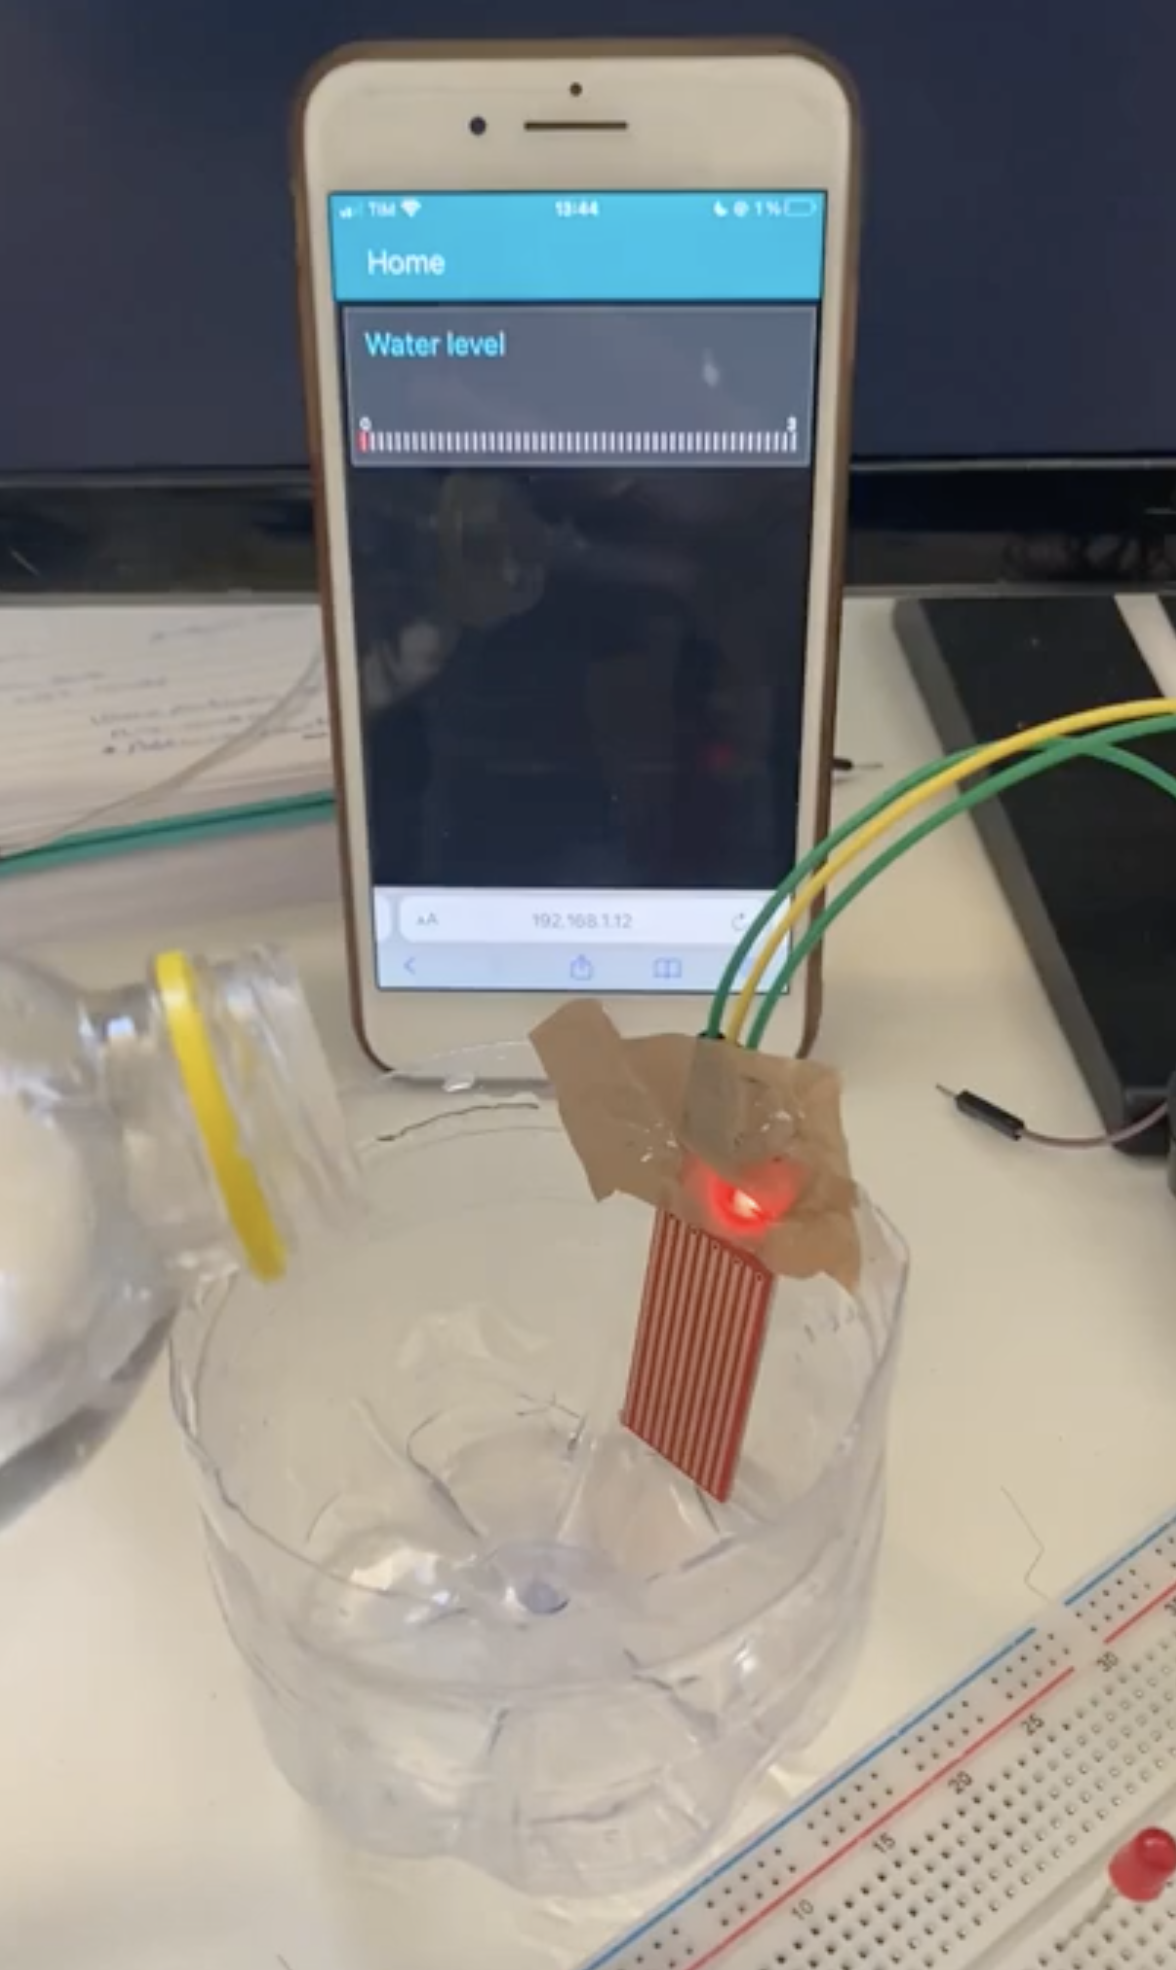
\includegraphics[width=3.4cm]{figs/agua1}}\hspace{1mm}
    \subfigure[]{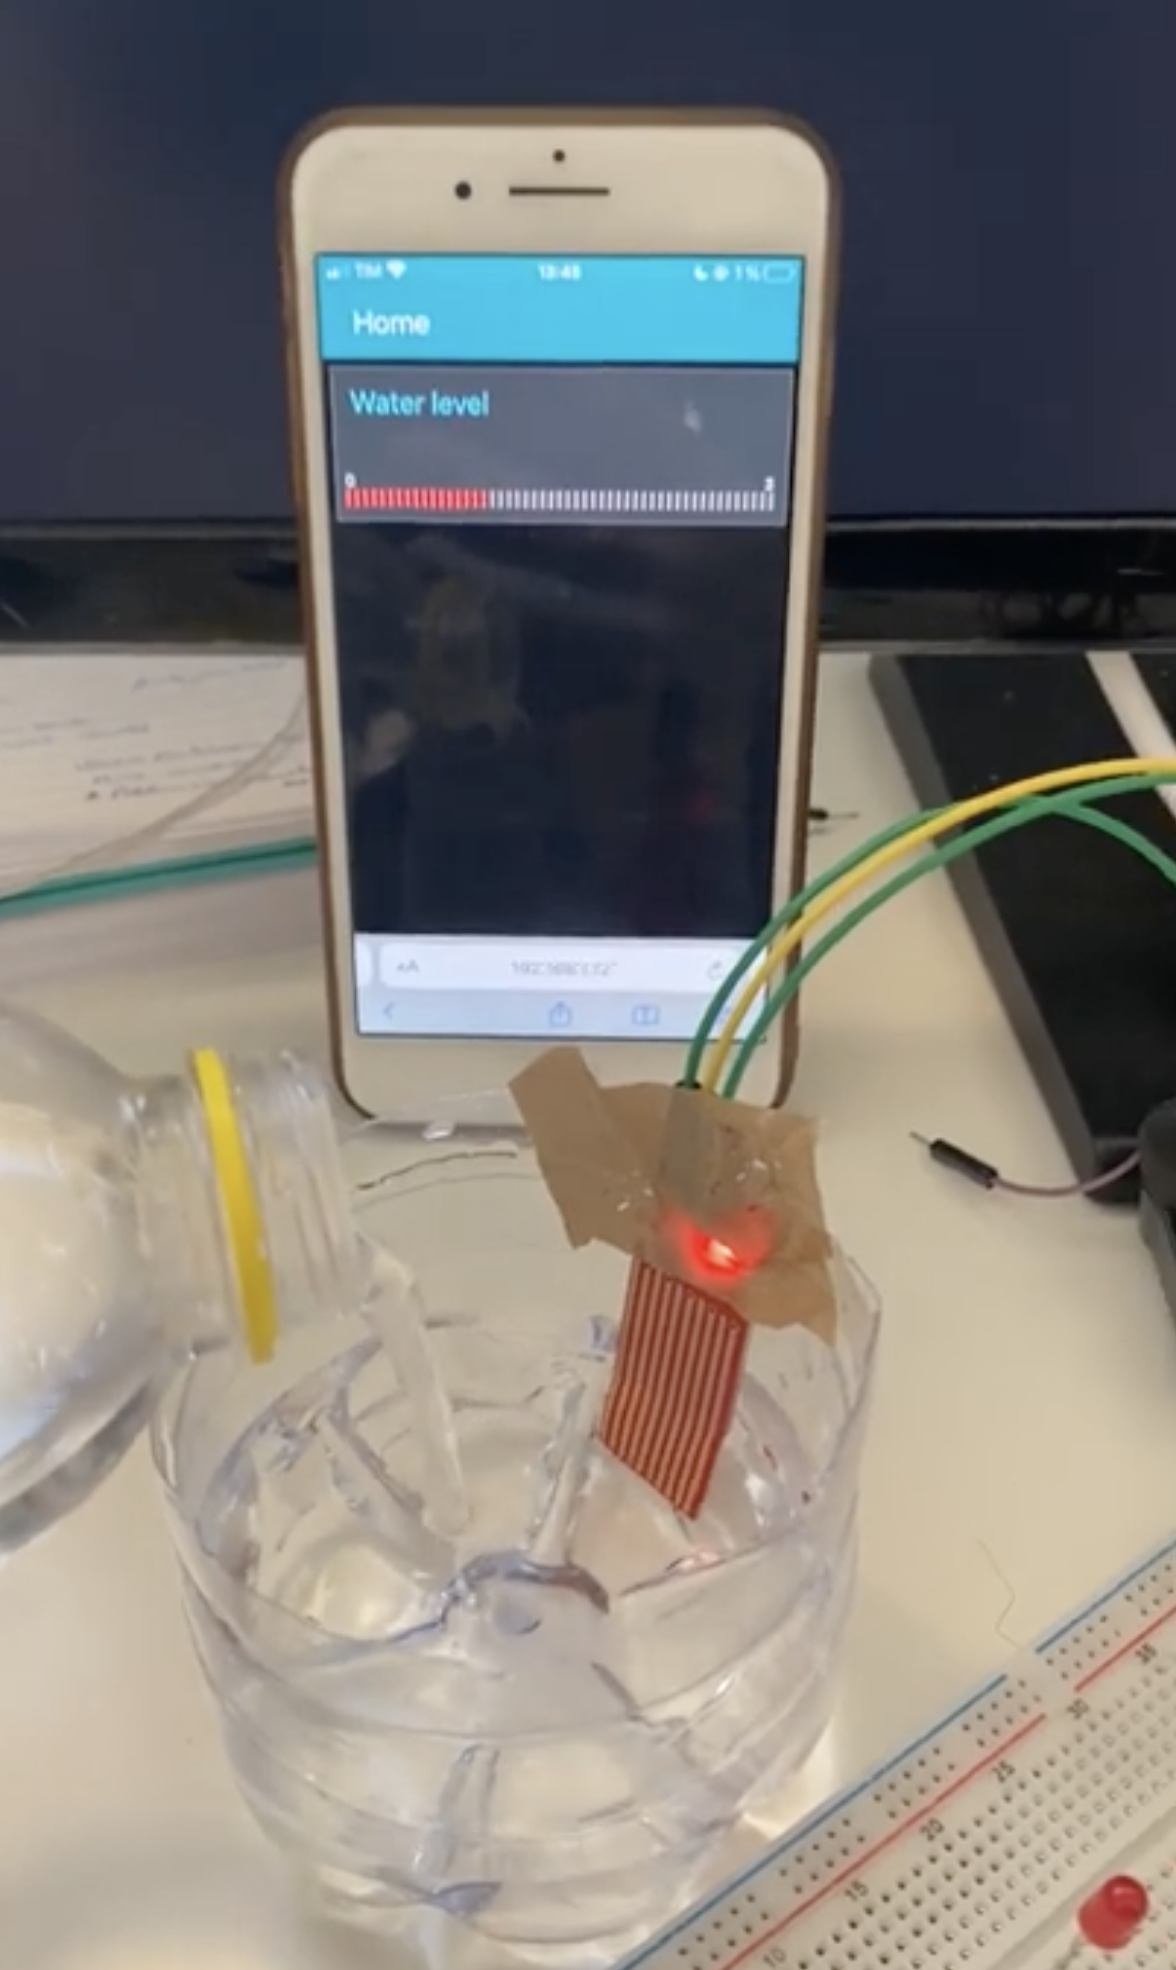
\includegraphics[width=3.4cm]{figs/agua2}}\hspace{1mm}
    \subfigure[]{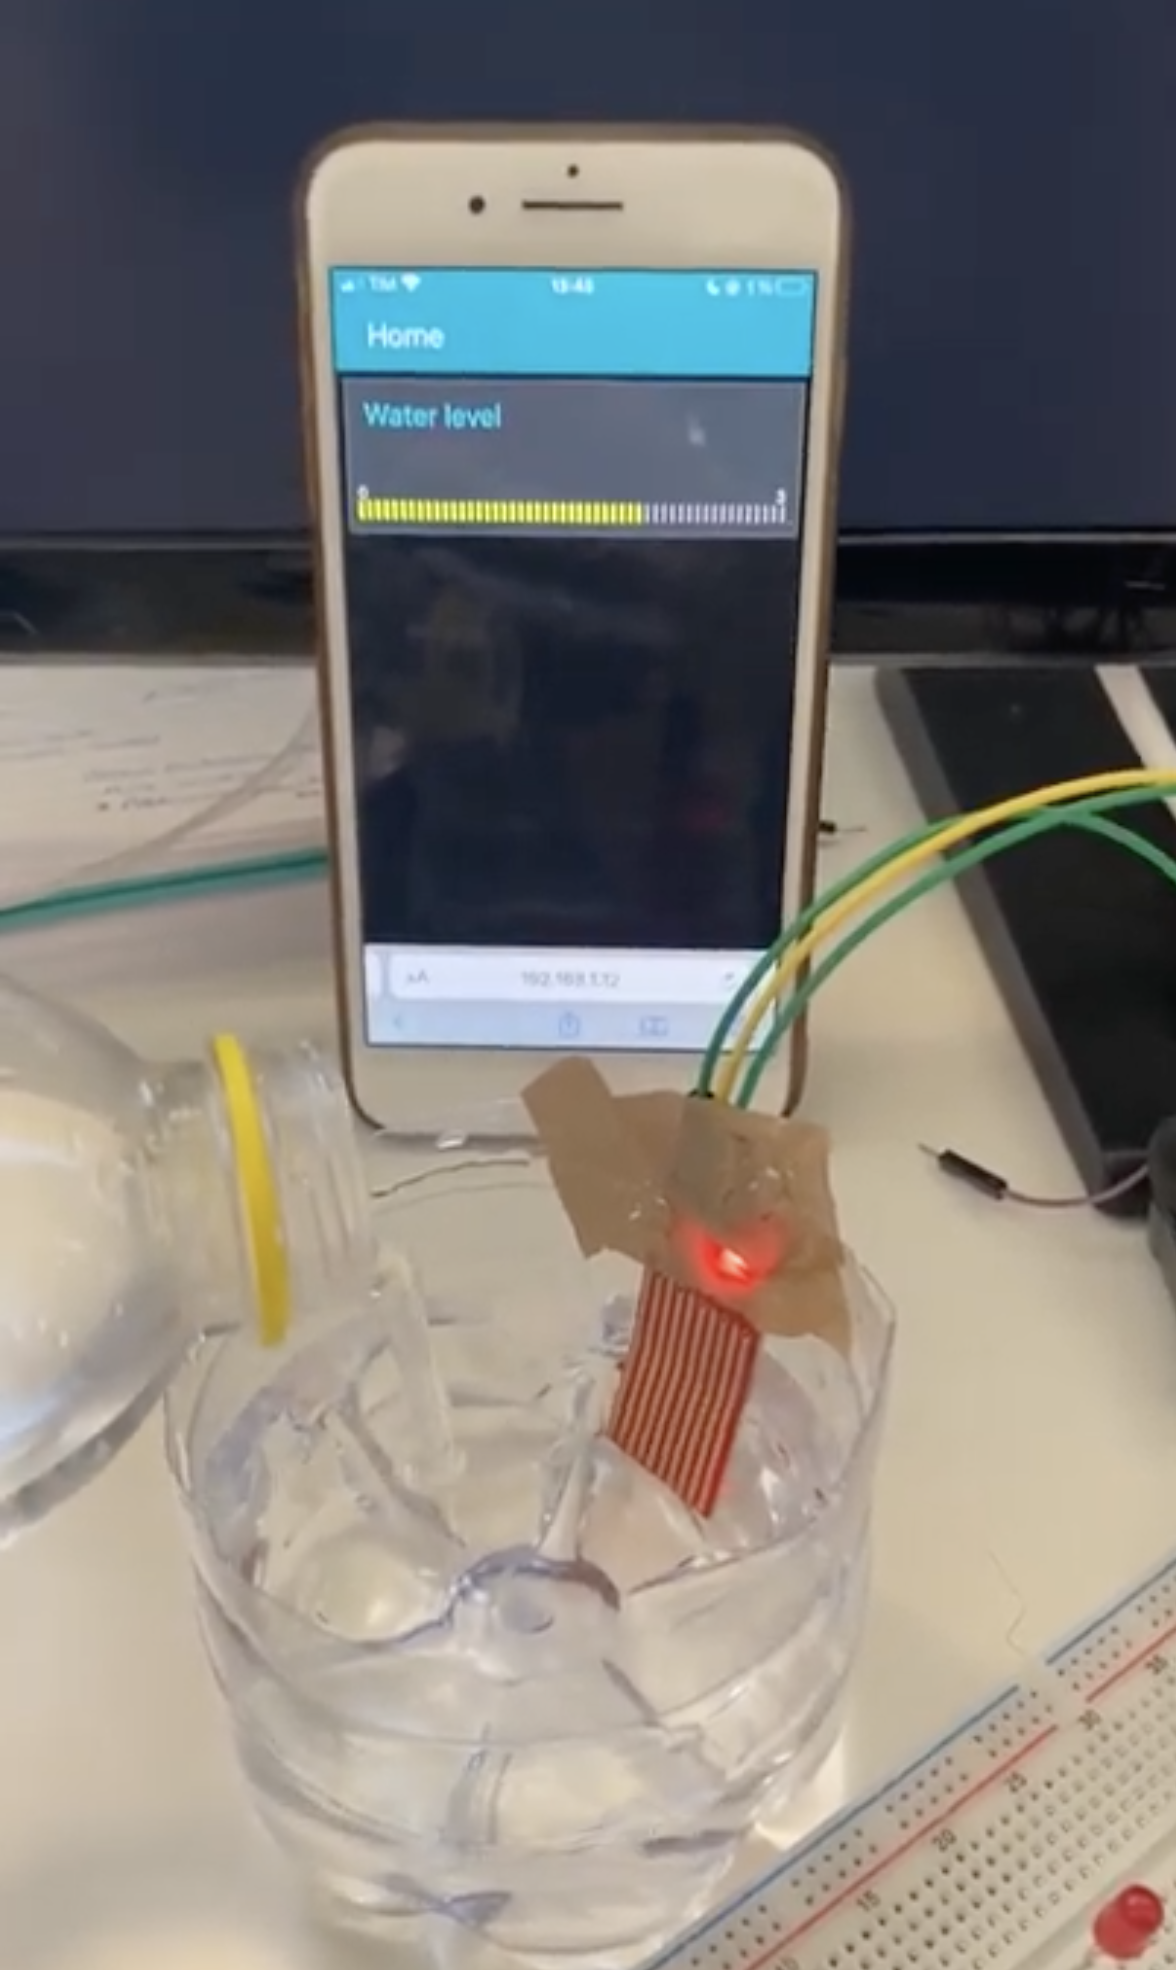
\includegraphics[width=3.4cm]{figs/agua3}}\hspace{1mm}
    \subfigure[]{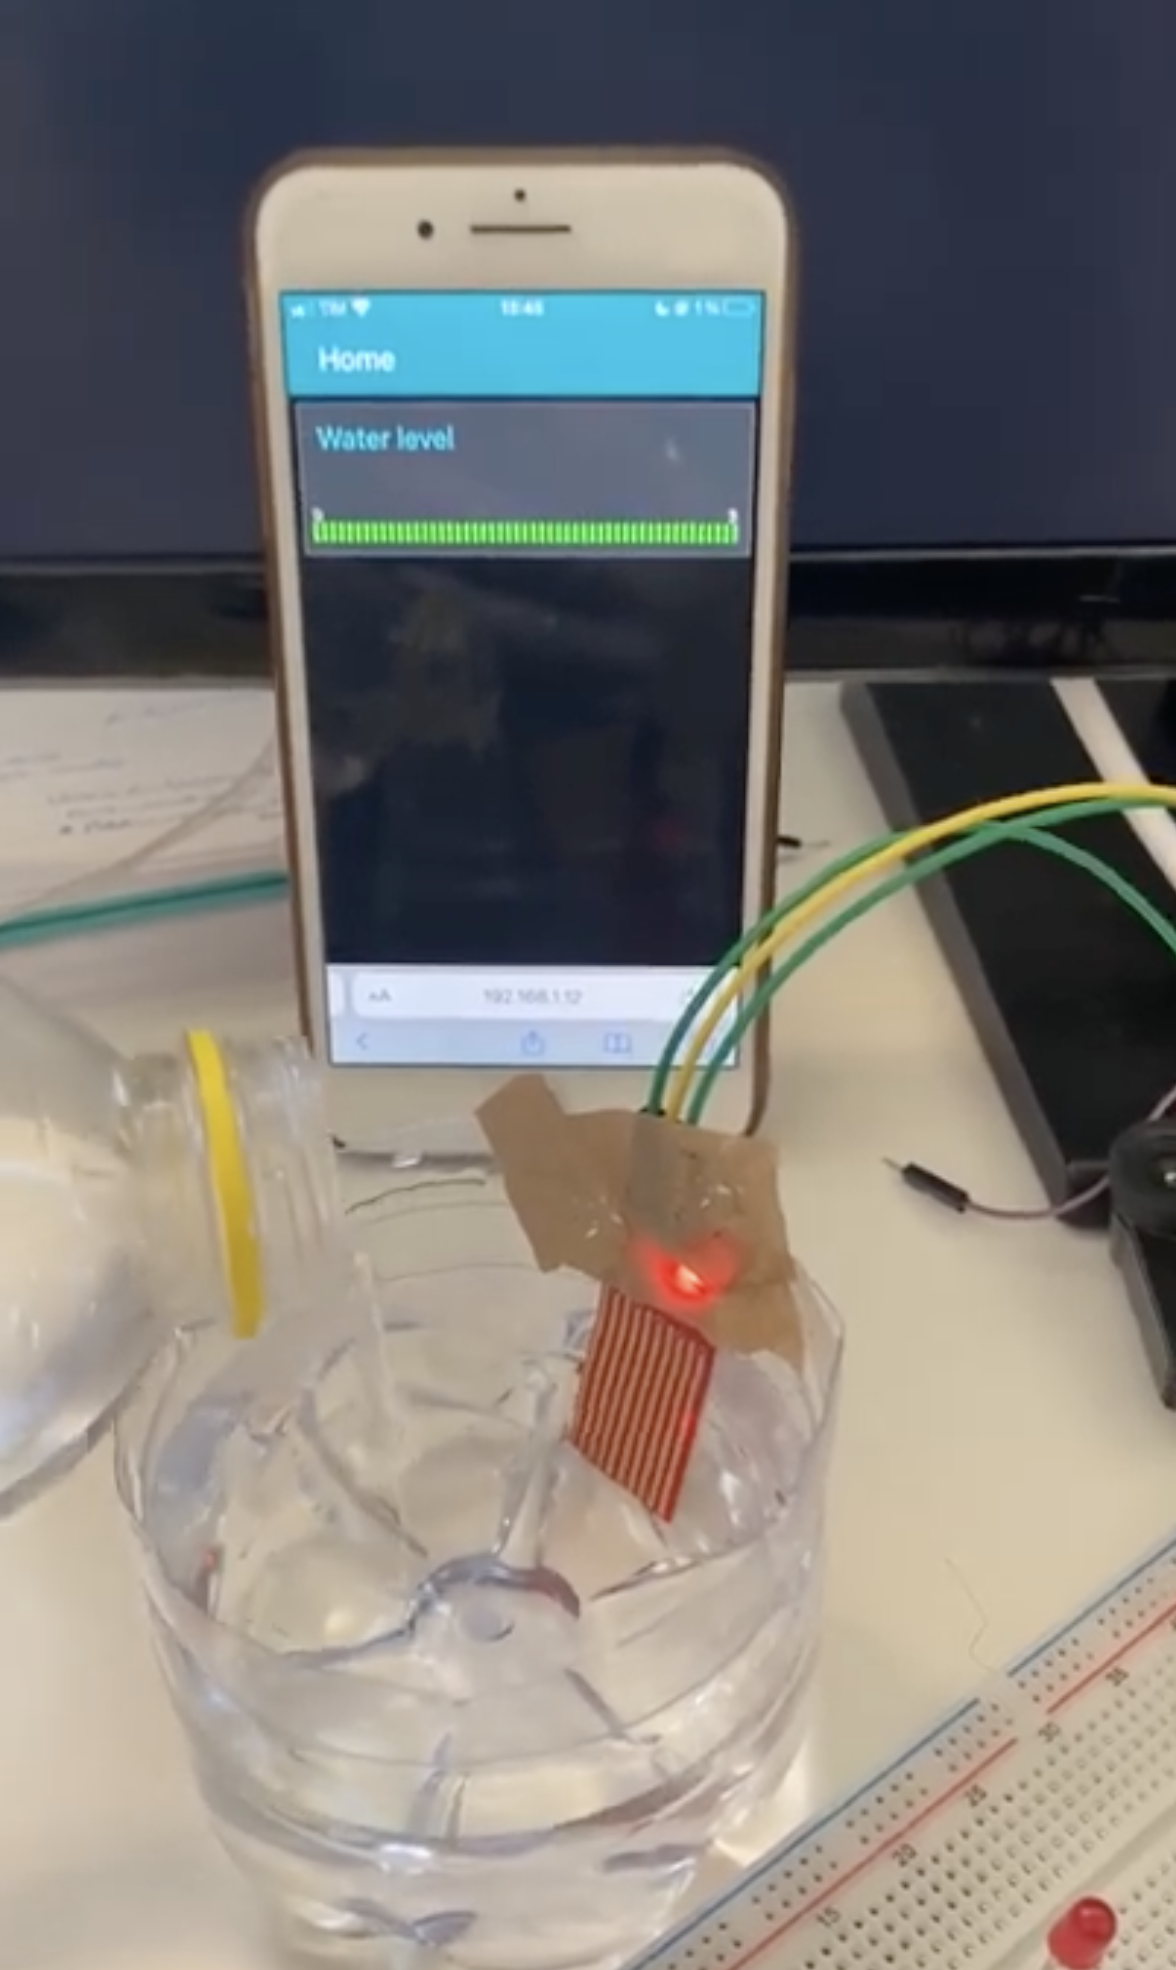
\includegraphics[width=3.4cm]{figs/agua4}}
  \end{center}
\caption{Proceso de indicación del nivel de agua.} \label{fig:agua}
\end{figure}

Con estos ajustes realizados, se ha obtenido parte de la IU. Para hacerla más completa se ha incorporado un interruptor de forma que el usuario puede decidir si apagarla o bien mantenerla encendida, así como un nodo que regula la repetitividad del sistema cada 3 segundos. La interfaz formada por los sensores comentados previamente se puede ver en la Figura \ref{fig:ui_nocams}.
\begin{figure} [h!]
  \begin{center}
    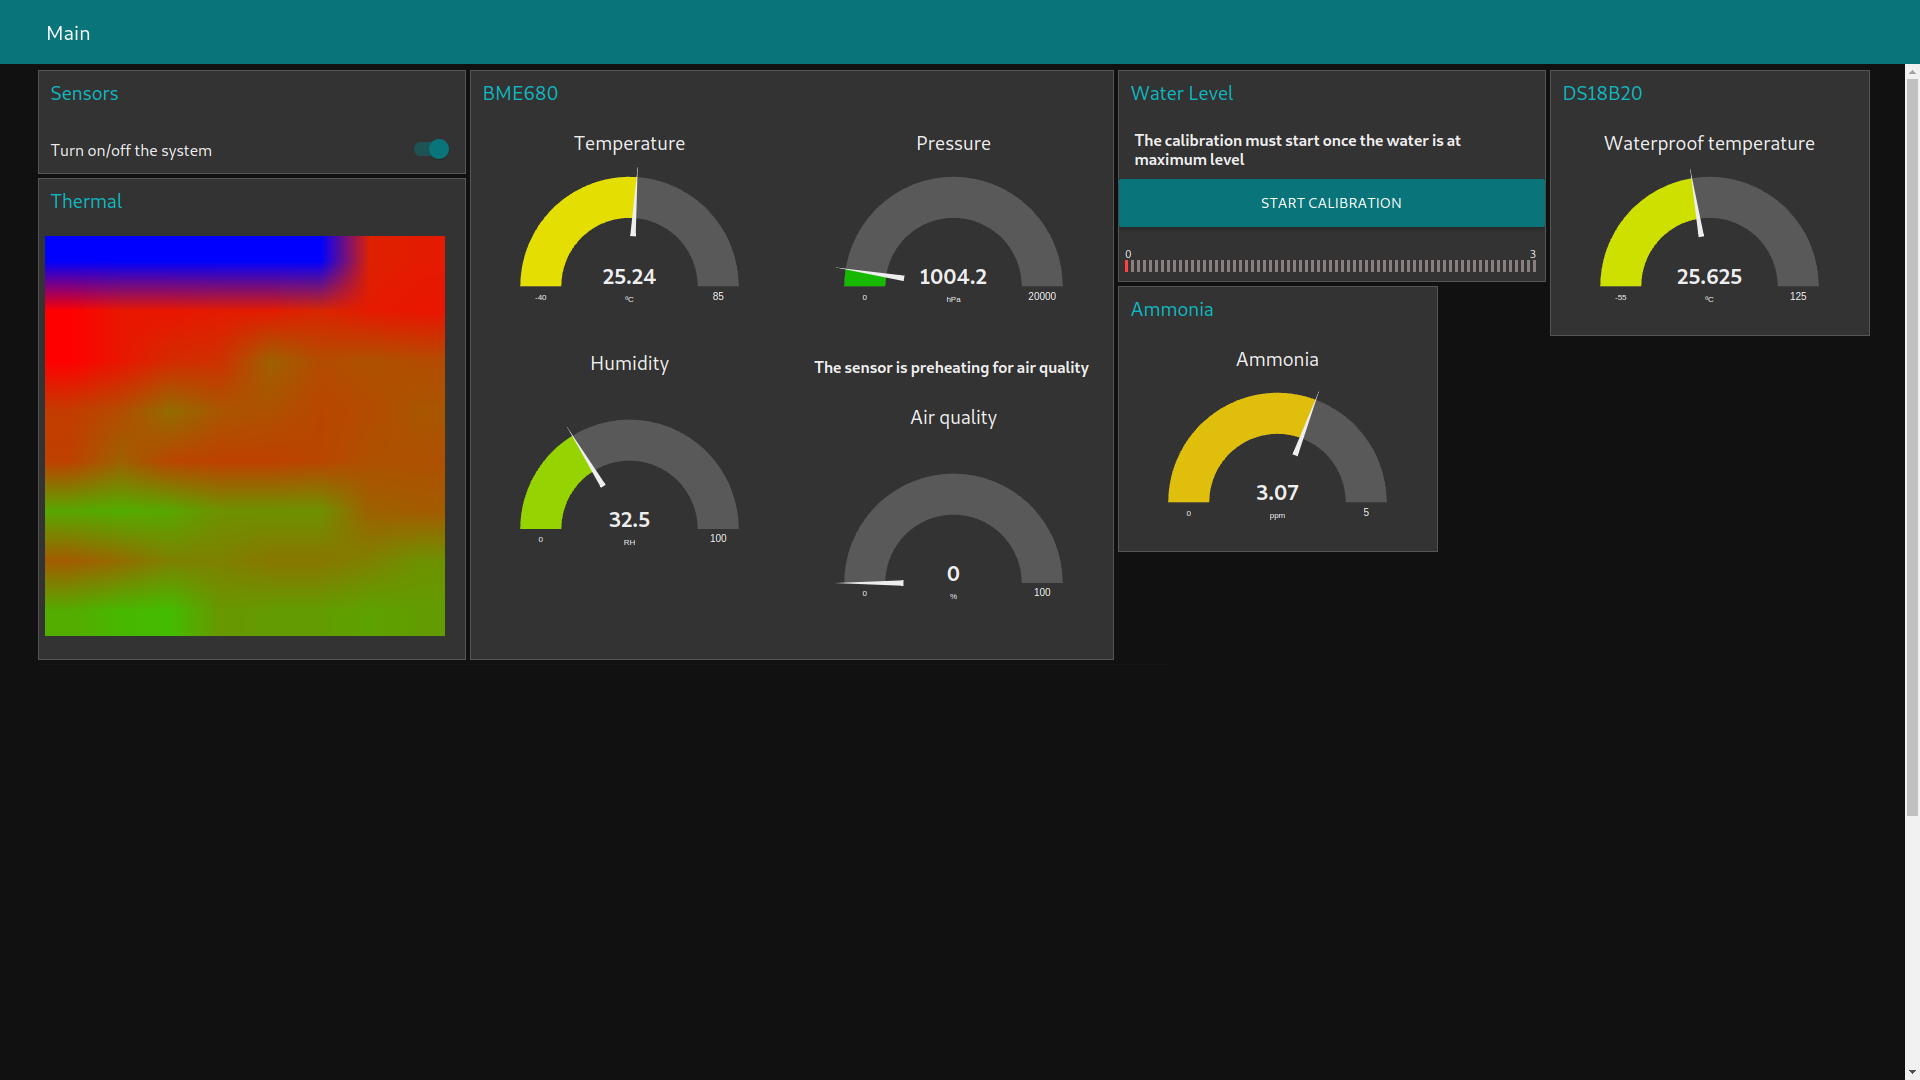
\includegraphics[width=16cm]{figs/ui_nocams}
  \end{center}
  \caption{IU sin los sensores cámaras.}
  \label{fig:ui_nocams}
\end{figure}

\subsection{Integración de las cámaras en la IU}
La creación de la interfaz en la subsección anterior no es completa, ya que faltan dos de los sensores que se utilizan en este trabajo: las cámaras. Para poder visualizar las cámaras desde Node-Red debe ser a través del nodo template (que significa plantilla), que permite visualizar una dirección web. Por tanto ha sido necesario crear un servidor que permita visualizar las imágenes de las dos cámaras y por tanto poder incluirlo en la IU. Para crear este servidor se ha utilizado Flask.\\

Se ha decidido crear un servidor por cada cámara. De esta manera se puede acceder solamente a una visualización o bien a las dos, según el interés del usuario. Para el funcionamiento de la cámara térmica Seek Thermal \ref{fig:termicos}-b se ha utilizado la librería que tiene seek, que permite su visualización a través de OpenCV. Para el funcionamiento de la PiCam \ref{fig:picam_of} se ha utilizado OpenCV tanto para su visualización como para la adición de la fecha y la hora en la visualización (Figura \ref{fig:fechayhora}). El código \ref{cod:fechayhora} muestra como se consigue.\\
\begin{figure} [h!]
  \begin{center}
    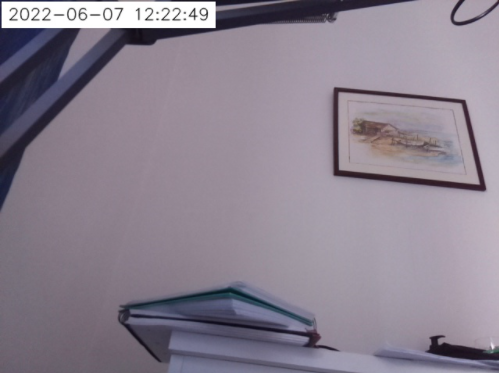
\includegraphics[width=8cm]{figs/fechayhora}
  \end{center}
  \caption{Incorporación de la fecha y hora en la visualización de la PiCam.}
  \label{fig:fechayhora}
\end{figure}

\begin{code}[h]
\begin{lstlisting}[language=Python]
ret, frame = self.__camera.read()
frame = cv2.rectangle(frame, (2,2), (275,35), (255,255,255), -1)
frame = cv2.putText(frame, str(datetime.datetime.now().replace(microsecond=0)), (10,25), cv2.FONT_HERSEY_SIMPLEX, 0.7, (0,0,0), 1, cv2.LINE_AA))
\end{lstlisting}
\caption[Código para incorporar la fecha en la esquina superior izquierda.]{Código para incorporar la fecha en la esquina superior izquierda.}
\label{cod:fechayhora}
\end{code}

Una vez obtenidas las imágenes de las cámaras desde la Raspberry, se ha incorporado al código el uso de Flask para poder crear el servidor. Es necesario disponer de dos elementos: el código para mostrar la imagen de la cámara y una carpeta donde estás las plantillas. Estas plantillas son ficheros escritos en html que muestran en el servidor la página que interesa en cada momento. La estructura que sigue un programa con Flask es la representada en el código \ref{cod:flask}.\\
\begin{code}[h]
\begin{lstlisting}[language=Python]
from flask import *
app = Flask(__name__)

@app.route('/')
def home():
   return render_template('index.html')

if __name__ == '__main__':
   app.run(host='0.0.0.0', port=8000, debug=True)
\end{lstlisting}
\caption[Código simple que crea un servidor web en el puerto 8000 y muestra el contenido de index.html.]{Código simple que crea un servidor web y muestra el contenido de index.html.}
\label{cod:flask}
\end{code}

Después de incorporar el código del funcionamiento de cada cámara en los respectivos servidores, se ha añadido un botón para iniciar o parar la grabación del vídeo en la cámara normal. Para diferenciar cuándo se está grabando de cuándo no, se ha añadido un mensaje en pantalla indicando que se está grabando. El vídeo se guarda en la Raspberry de forma local y en formato .avi. En la Figura \ref{fig:proceso} se puede ver el proceso de registro en el servidor para acceder a la visualización de la PiCamera.\\
\begin{figure}[h!]
  \begin{center}
    \subfigure[Pantalla inicial del servidor]{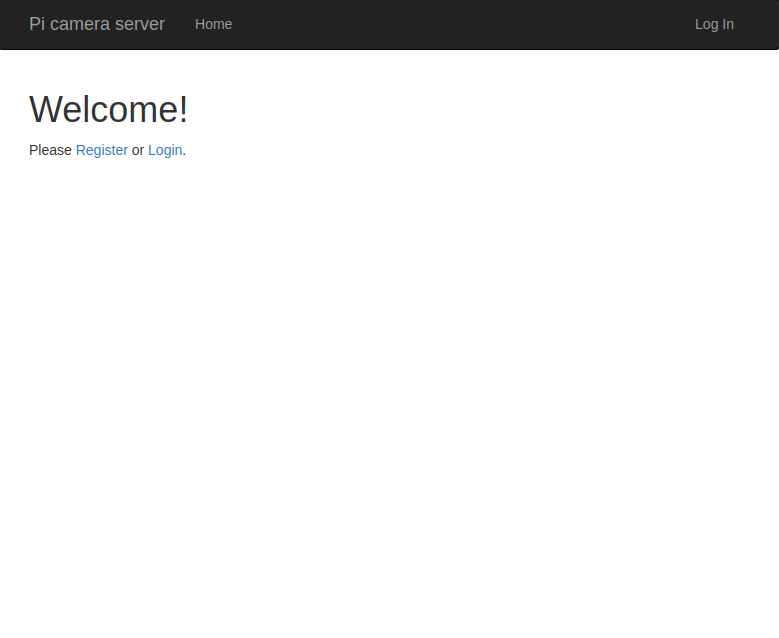
\includegraphics[width=7cm]{figs/server1}}\hspace{1mm}
    \subfigure[Pantalla de registro]{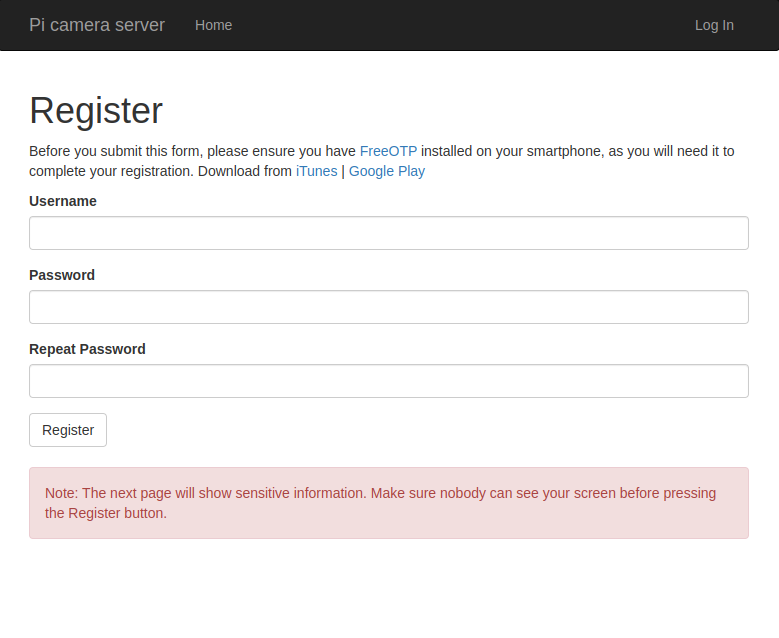
\includegraphics[width=7cm]{figs/server2}}\hspace{2mm}
    \subfigure[Código de doble autenticación]{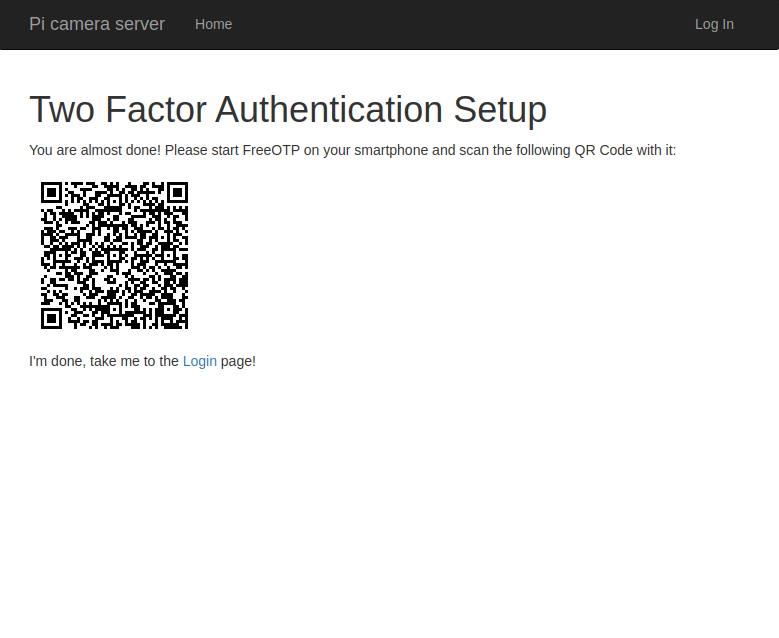
\includegraphics[width=7cm]{figs/server3}}\hspace{1mm}
    \subfigure[Escaneo de código]{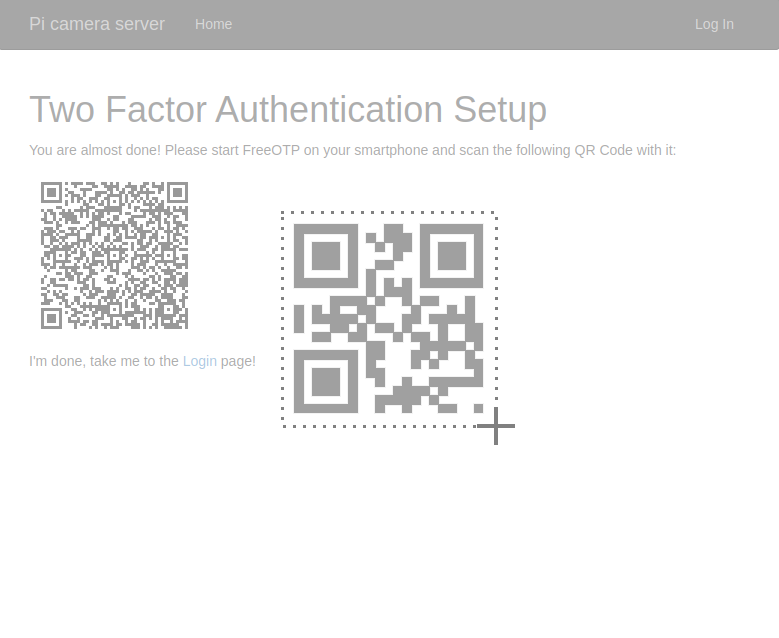
\includegraphics[width=7cm]{figs/server4}}
    \subfigure[Pantalla de login]{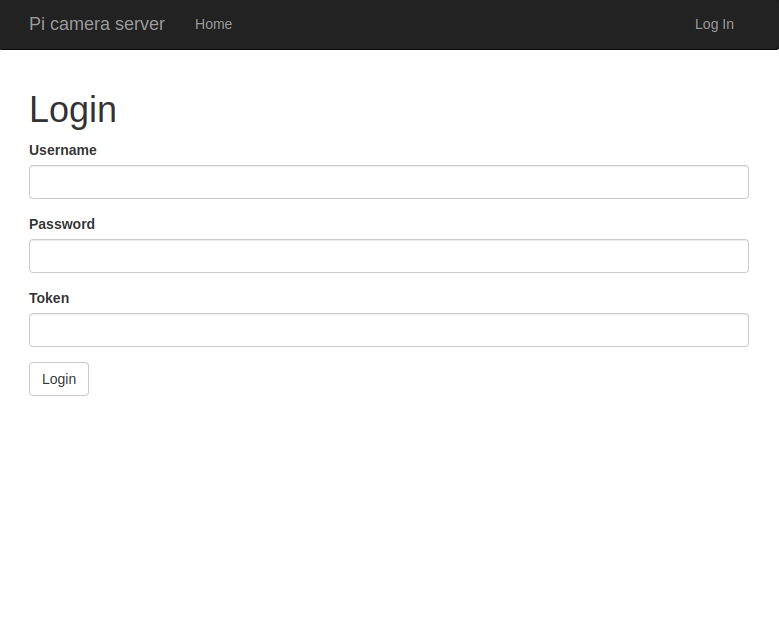
\includegraphics[width=7cm]{figs/server6}}\hspace{2mm}
    \subfigure[Visualización de la cámara]{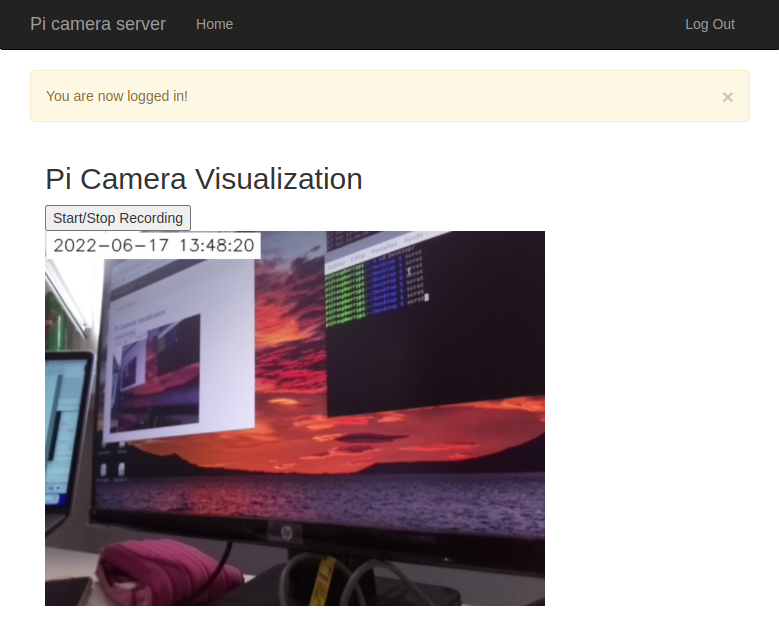
\includegraphics[width=7cm]{figs/server7}}
  \end{center}
\caption{Proceso de registro en el servidor de Flask de la PiCam.} \label{fig:proceso}
\end{figure}

Una vez se ha obtenido la visualización de las cámaras en la IU junto al resto de sensores, la interfaz está completada siguiendo la estructura presentada en el diagrama de casos de uso (Figura \ref{fig:casos}).


\subsection{Seguridad}
Debido a que se está trabajando en un servidor web, es importante dotar de cierta seguridad al servidor para evitar que sólo las personas autorizadas puedan acceder a las imágenes. Para ello, se ha decidido hacerlo a través del factor de doble autenticación (del inglés two factor authentication, 2FA). 2FA es el proceso de autenticación donde se añade un segundo paso en el proceso de identificación frente a un servicio. En este caso, además de que un usuario introduzca su contraseña, es necesario un código que se genera cada 30 segundos y caduca pasado ese tiempo. La generación de este código se hace a través de google authenticator \footnote{\url{https://chrome.google.com/webstore/detail/authenticator/bhghoamapcdpbohphigoooaddinpkbai?hl=es}}. Esta extensión de google genera los códigos de 30 segundos a partir de el escaneo de un código QR (Figura \ref{fig:server}-d) o por la inserción manual de un código inicial.\\

Para que estos servidores funcionen con 2FA, ha sido necesario incorporar otras librerías así como otros módulos de Flask como Flask\_login, Flask\_bootstrap, Flask\_sqlalchemy o Flask\_wtf. Durante el desarrollo del servidor con 2FA, han surgido determinados problemas que pueden encontrarse junto a la solución en la wiki del proyecto \footnote{\url{https://github.com/jmvega/tfg-icebollada/wiki/5.May-progress}}.\\

Una vez los servidores web han funcionado, se han integrado en Node-Red a través del nodo template. Un servidor está en el puerto 5000 y el otro en el 8000 para que así puedan estar ambas cámaras disponibles a la vez. Después de añadirlos, la interfaz de usuario (Figura \ref{fig:UIcompleta}) se ha completado.\\
\begin{figure} [h!]
  \begin{center}
    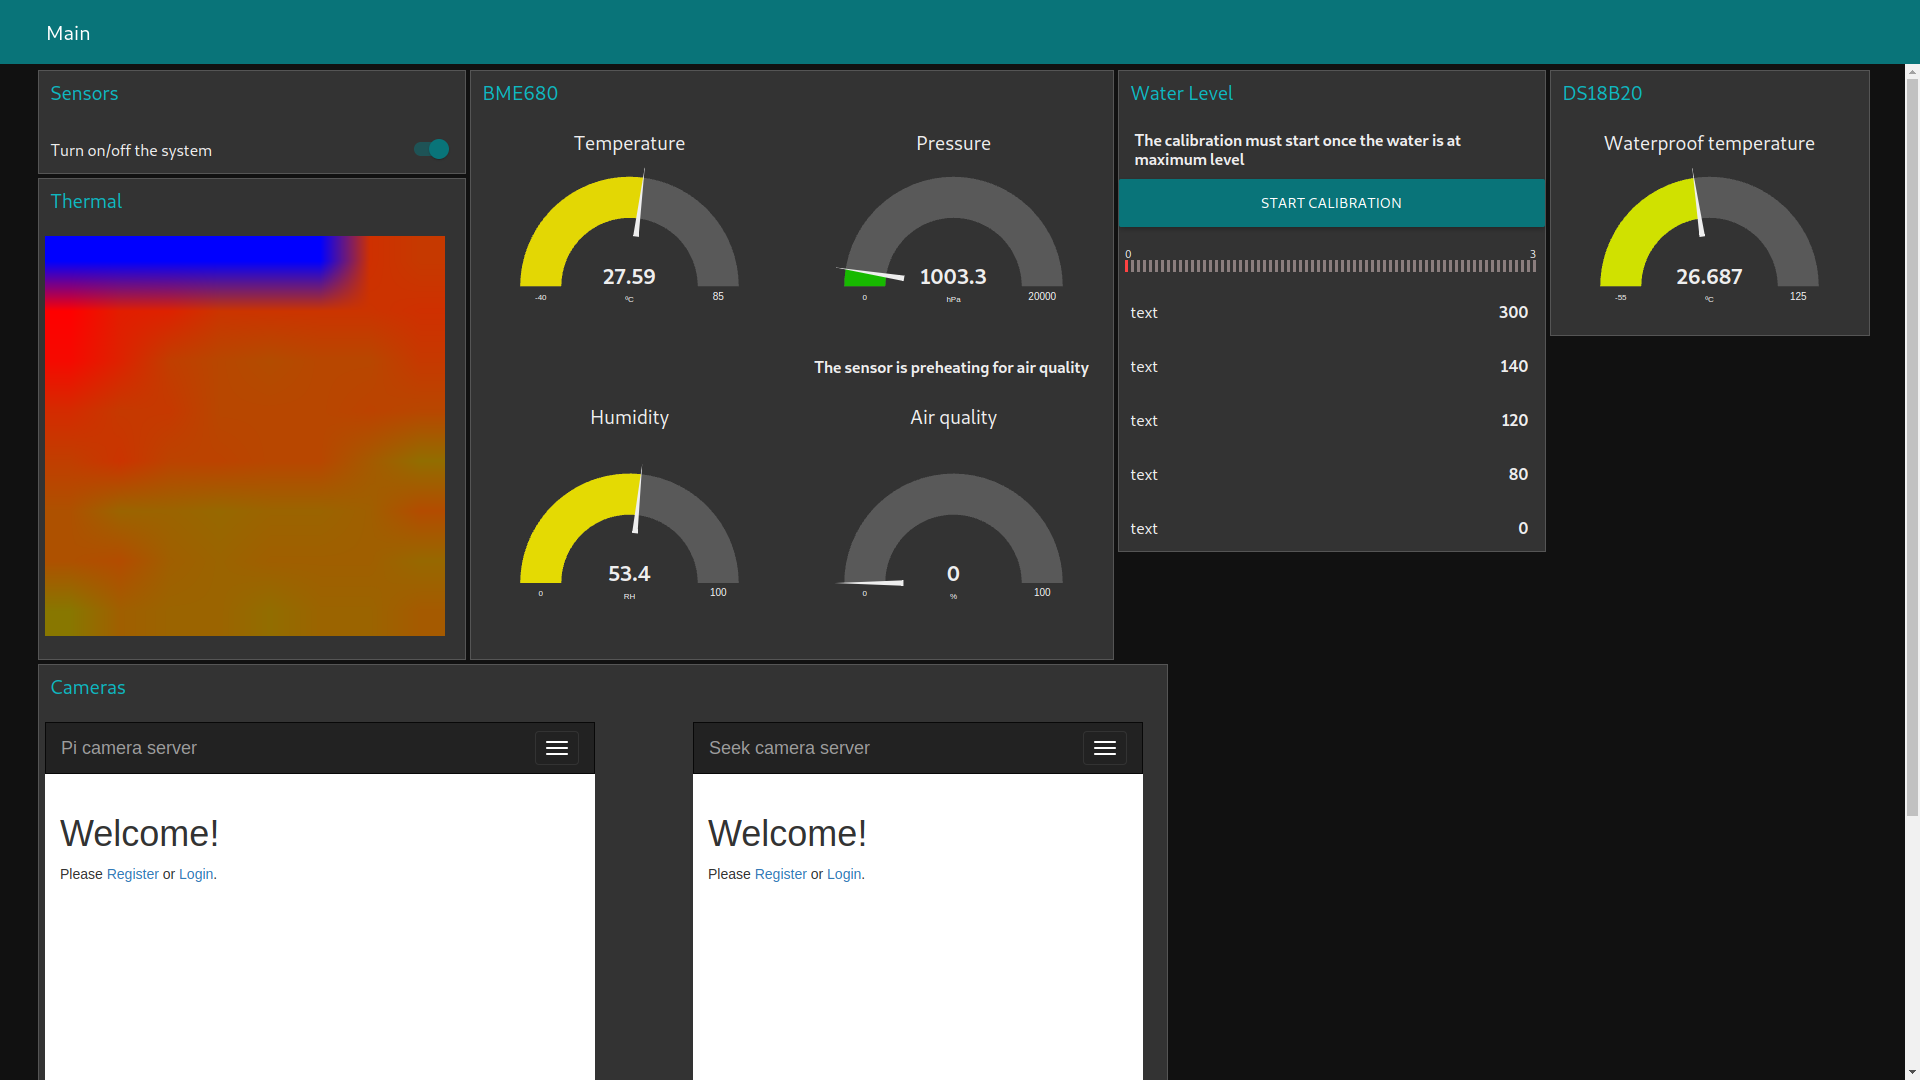
\includegraphics[width=16cm]{figs/UIcompleta}
  \end{center}
  \caption{Visualización de la interfaz de usuario.}
  \label{fig:UIcompleta}
\end{figure}

También se ha tenido en cuenta que Node-Red funciona sobre una dirección a la que puede acceder cualquier usuario de la red sobre el puerto 1880. Por tanto, es imprescindible que sean solo usuarios autorizados los que puedan acceder a esta plataforma, sobre todo en la parte del flujo de nodos. Por tanto se ha optado por dividir este acceso en dos partes: Una de ellas la parte de administrador (Figura \ref{fig:adminlogin}), donde se encuentra el flujo de nodos y se crea toda la interfaz de usuario. Únicamente un administrador debe poder acceder a esta parte, ya que es importante que una persona que no tiene conocimientos acerca de su funcionamiento no pueda realizar modificaciones. La otra parte corresponde a la interfaz de usuario (Figura \ref{fig:userlogin}) que, aunque ahí no pueden realizarse modificaciones, solo un usuario registrado conocedor de la contraseña sea capaz de acceder para evitar que personas ajenas puedan acceder a la información disponible.\\
\begin{figure} [h!]
  \begin{center}
    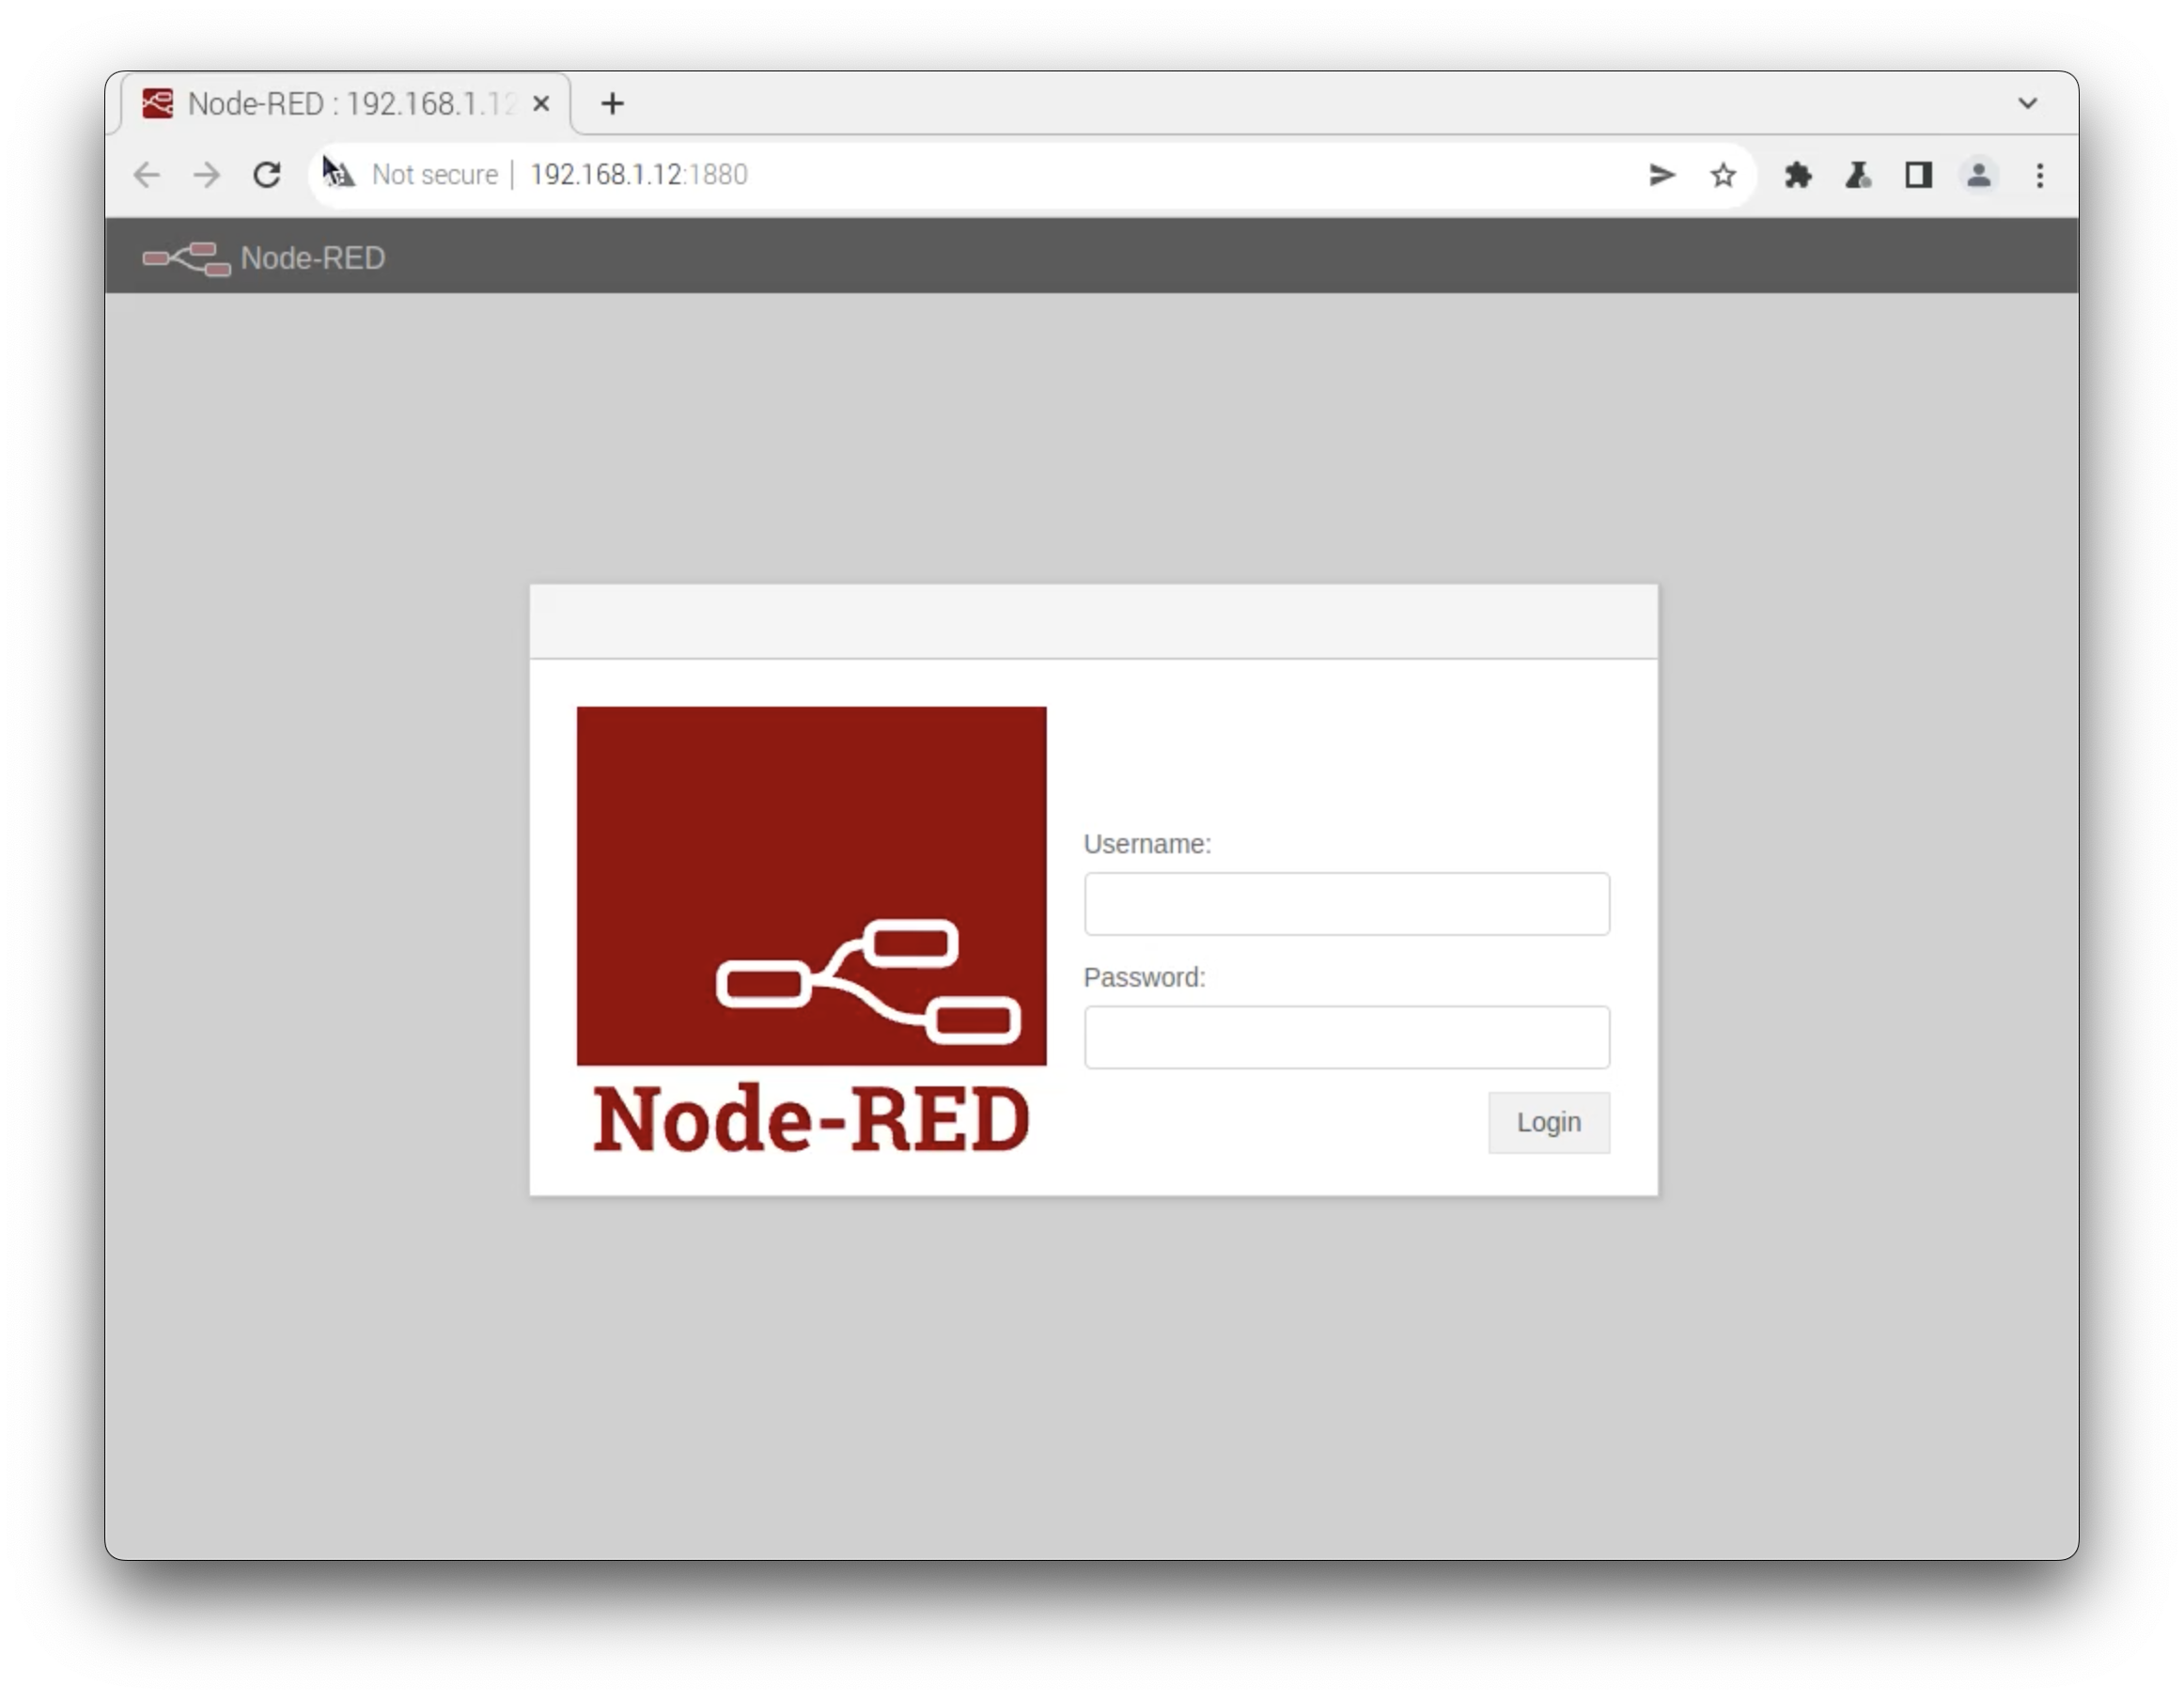
\includegraphics[width=12cm]{figs/adminlogin}
  \end{center}
  \caption{Acceso al flujo de nodos en Node-Red.}
  \label{fig:adminlogin}
\end{figure}

\begin{figure}[h!]
  \begin{center}
    \subfigure[]{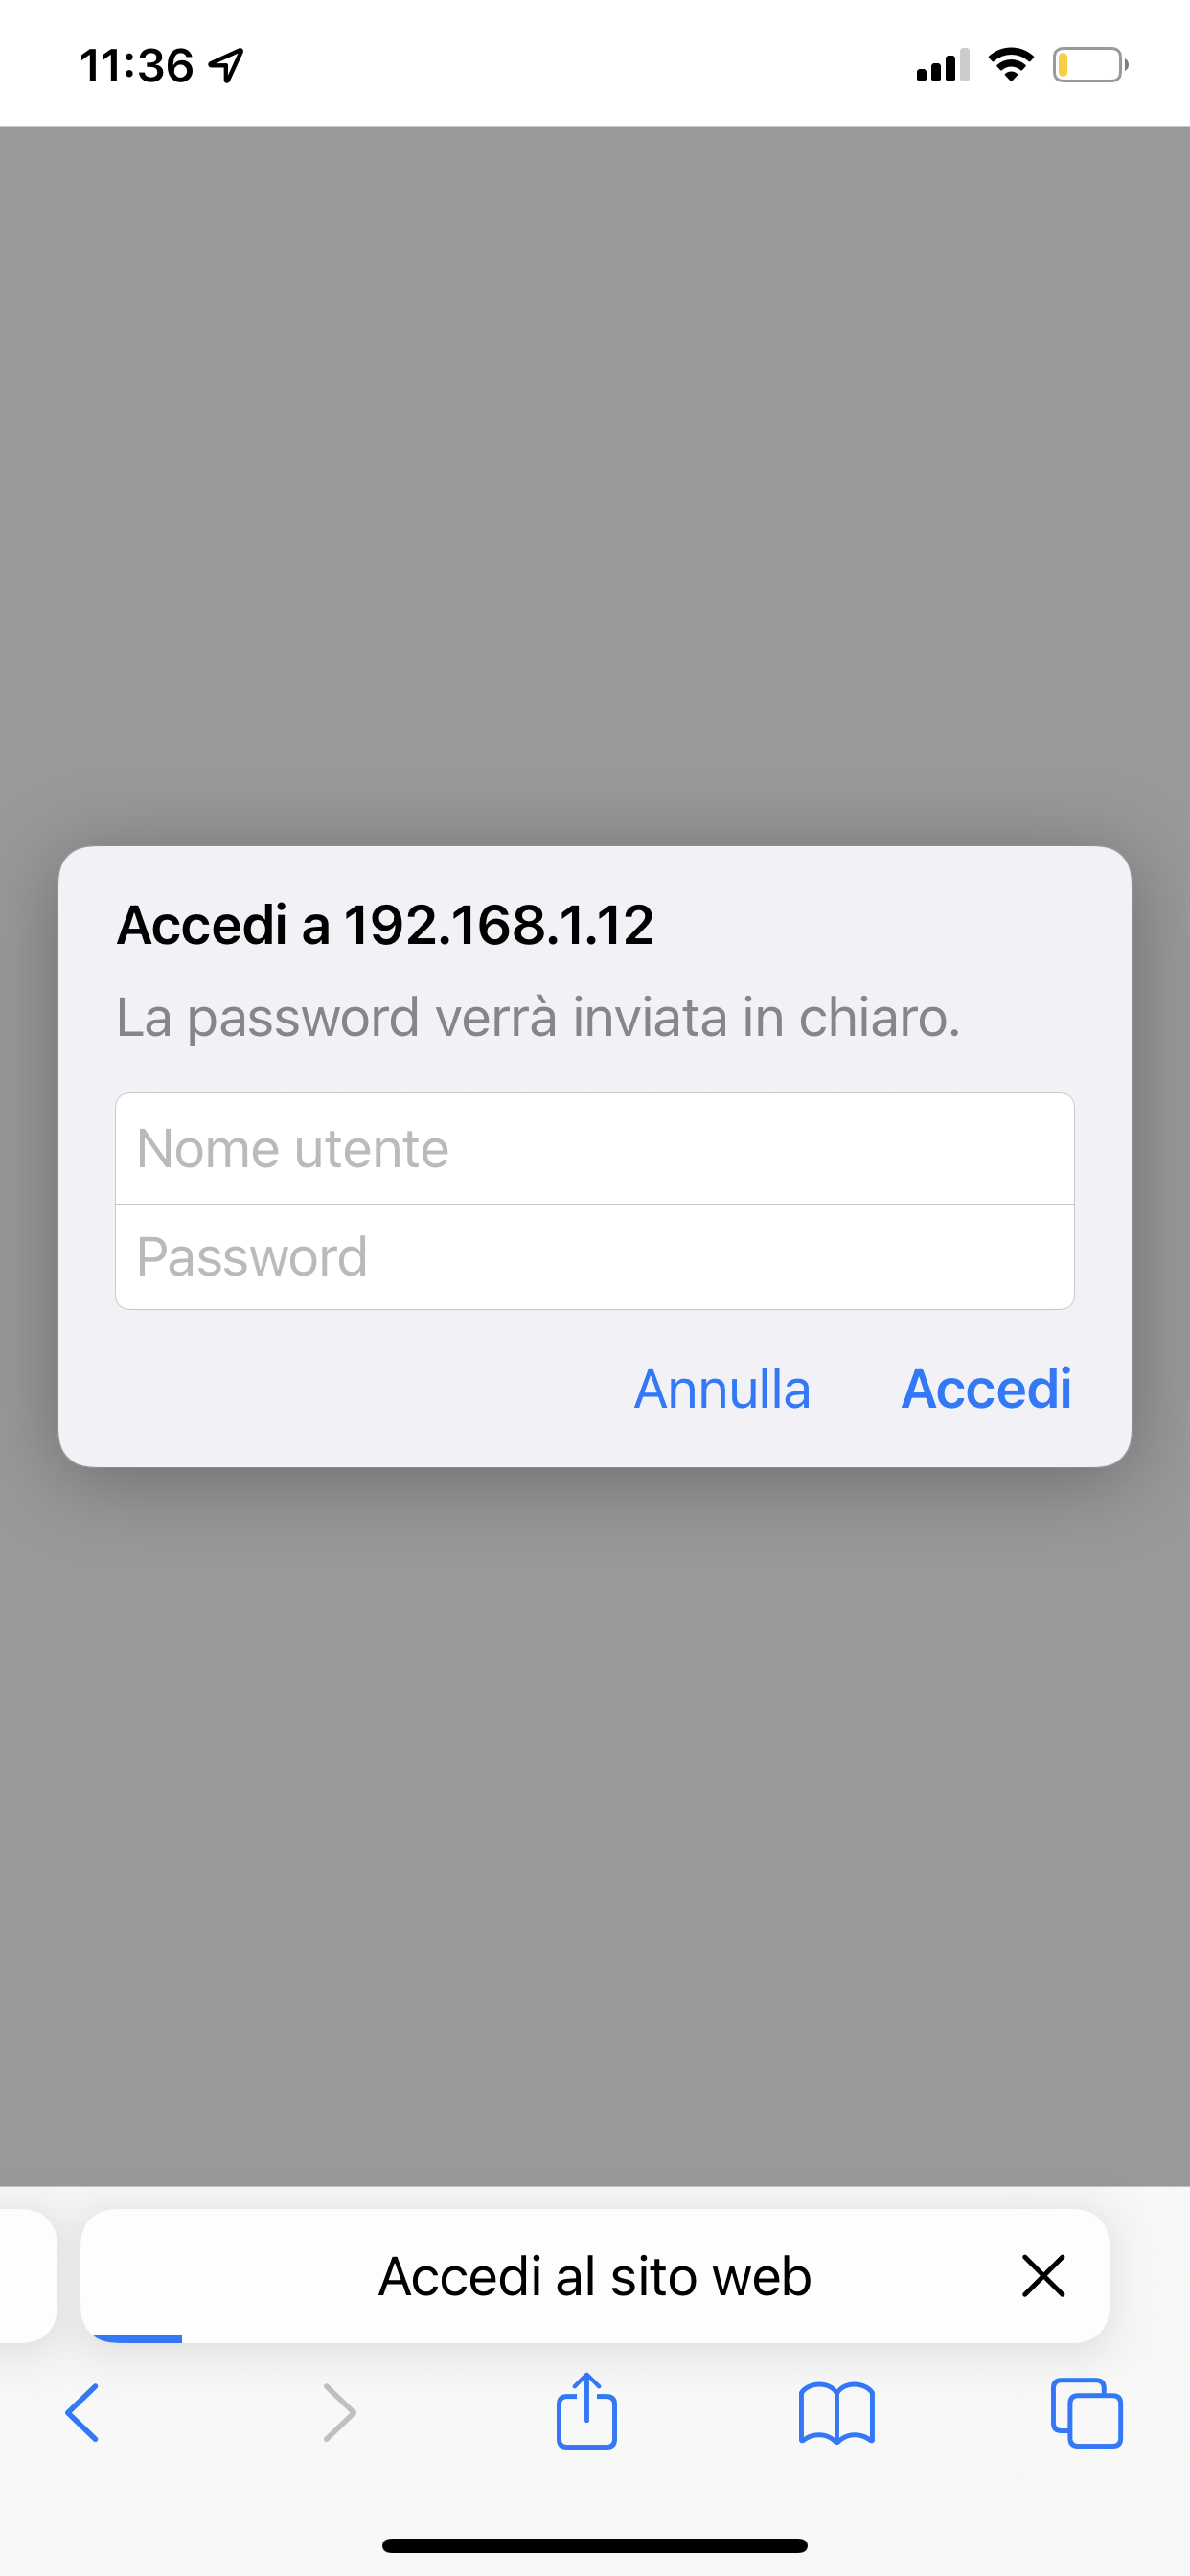
\includegraphics[width=60mm]{figs/phonelogin}}\hspace{2mm}
    \subfigure[]{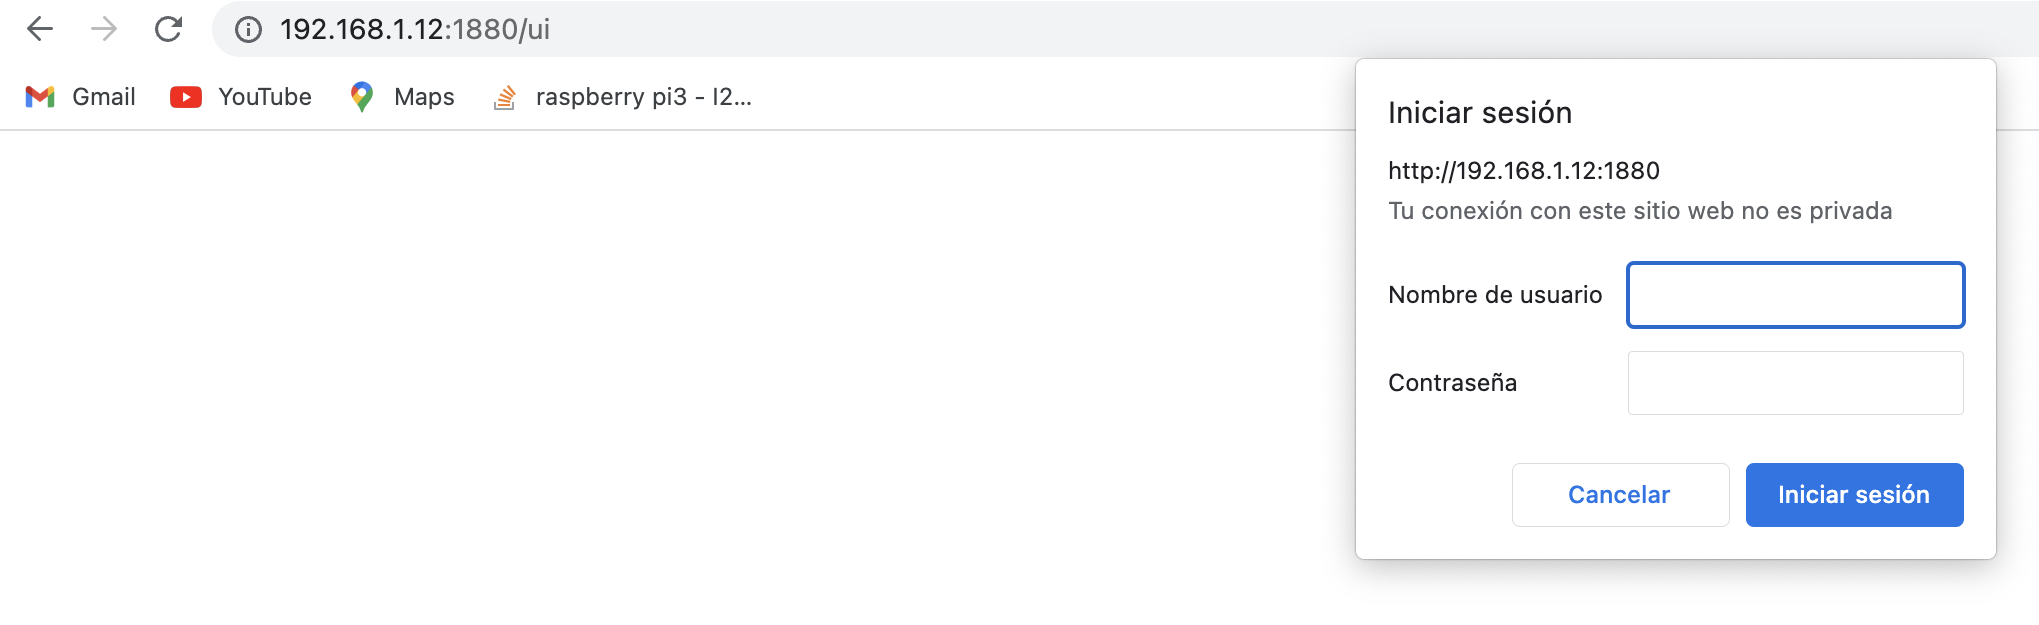
\includegraphics[width=150mm]{figs/maclogin}}
  \end{center}
\caption{Acceso a la interfaz de usuario desde distintos dispositivos.} \label{fig:userlogin}
\end{figure}

Tanto las contraseñas de Node-Red como las de los servidores se guardan encriptadas bajo algoritmos de funciones hash en SHA256.\\

Por otro lado, tanto los servidores de Flask como Node-Red se encontraban bajo una URL de HTTP (Hypertext Transfer Protocol). Por tanto, un cambio necesario ha sido añadir seguridad de tal forma que sea HTTPS (Hypertext Transfer Protocol Secure), para impedir que otros usuarios puedan interceptar la información confidencial que se transfiere entre el cliente y los servidores web a través de Internet. Este cambio se ha realizado añadiendo certificados autofirmados creados por el autor.\\

\subsection{Autoarranque}
Recordando que este sistema está pensado para personas que no están familiarizadas con la programación o los ordenadores, se ha considerado añadir una opción que facilite el arranque del sistema.\\

Con el encendido de la Raspberry, la interfaz de usuario se lanza de forma automática ---así como los dos servidores--- y se enciende solicitando el login del usuario para acceder a la IU. Además, se ha incorporado un led verde que indica cuando el sistema está listo para ser usado. El funcionamiento del autoarranque, tanto de Node-Red como de los servidores se encuentra detallado en la wiki \footnote{\url{https://github.com/jmvega/tfg-icebollada/wiki/5.May-progress}}. El proceso de autoarranque es visible en la Figura \ref{fig:autoarranque}.
\begin{figure}[h!]
  \begin{center}
    \subfigure[Encendido de la Raspberry]{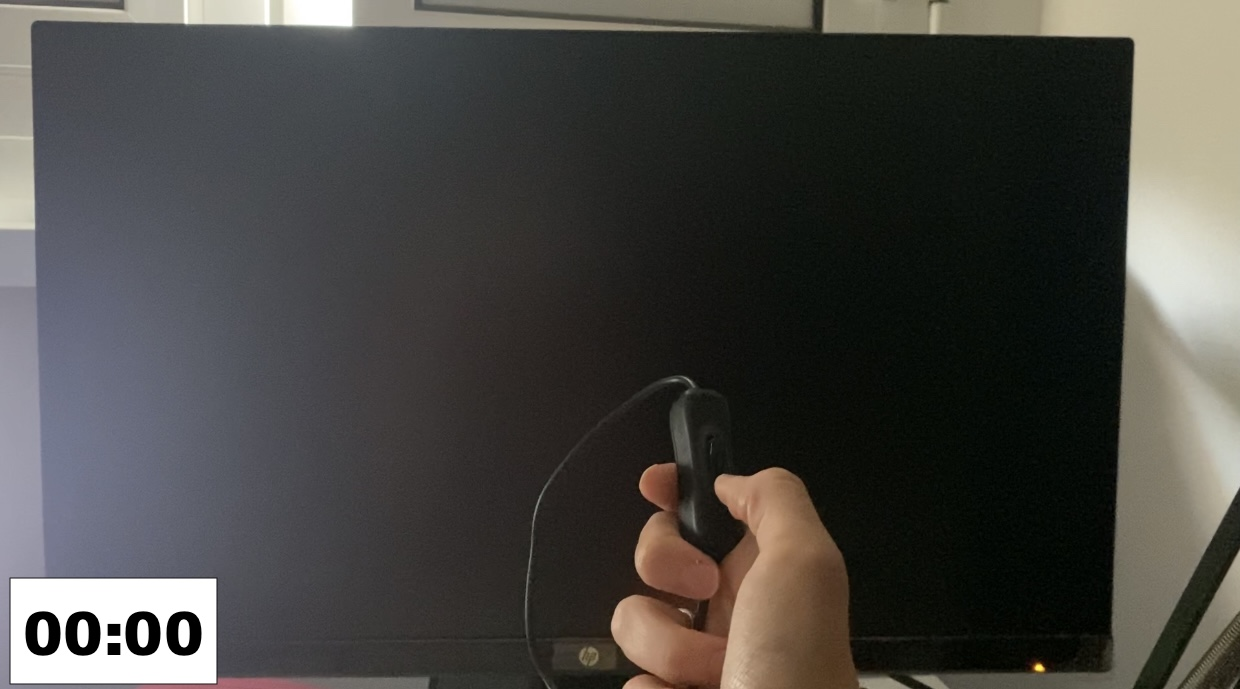
\includegraphics[width=7cm]{figs/auto1}}\hspace{1mm}
    \subfigure[]{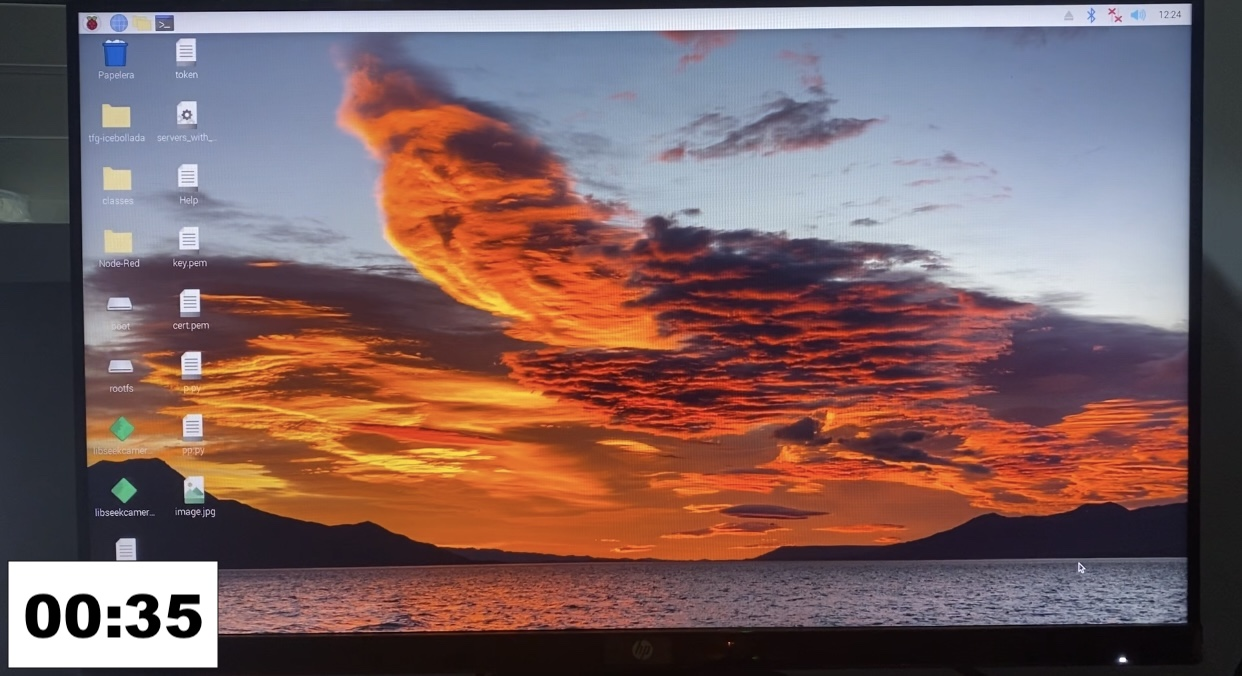
\includegraphics[width=7.2cm]{figs/auto2}}\hspace{1mm}
    \subfigure[]{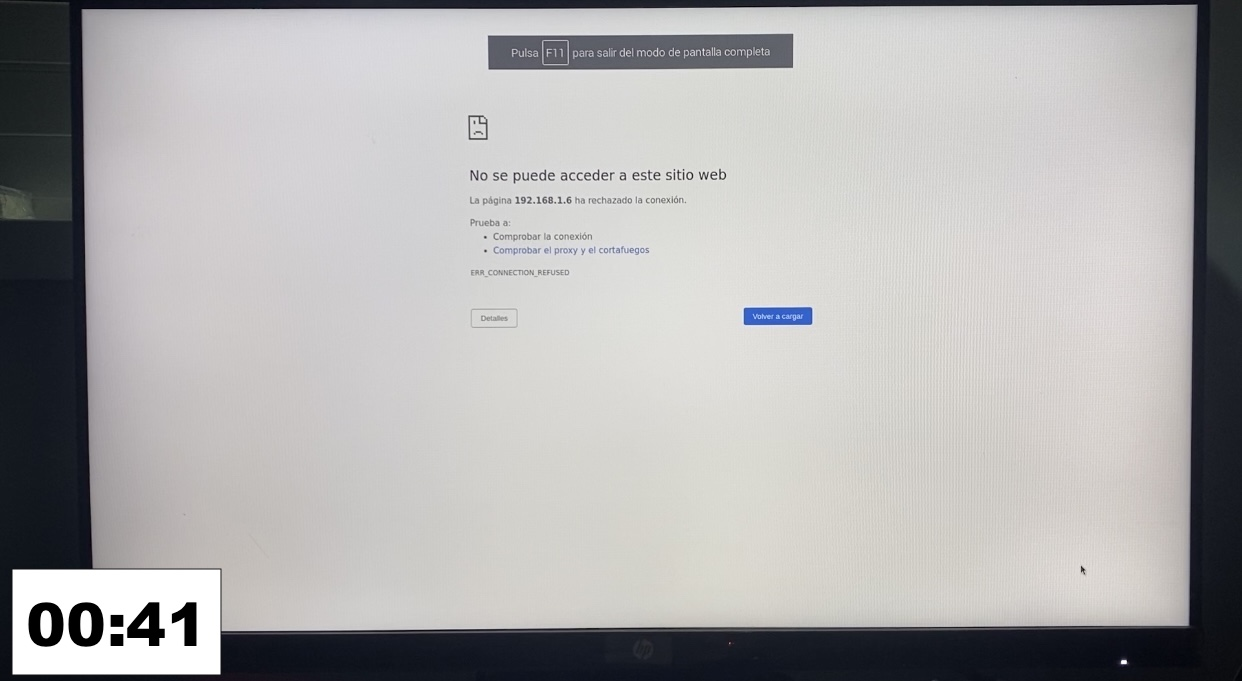
\includegraphics[width=7cm]{figs/auto3}}\hspace{1mm}
    \subfigure[Sistema listo para iniciar sesión]{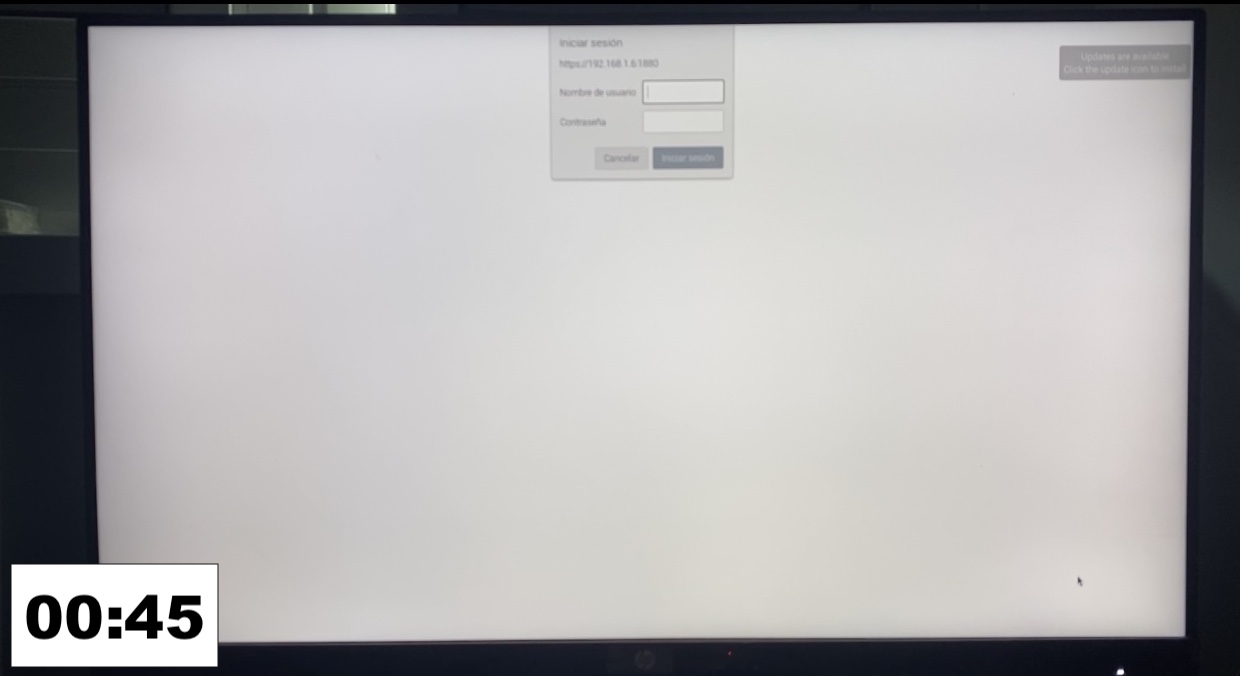
\includegraphics[width=7.1cm]{figs/auto4}}
  \end{center}
\caption{Proceso de autoarranque del sistema.} \label{fig:autoarranque}
\end{figure}

\subsection{Detección de ratones con uso de Deep Learning}
Finalmente para el cumplimiento del tercer objetivo era necesaria la detección de ratones. Para ello, ha sido necesaria la creación de un dataset de ratones, debido a que no se ha encontrado ninguno en internet. Está formado 354 imágenes; 275 para el proceso de entrenamiento y 79 para el de validación. El puede encontrarse en la plataforma Kaggle \footnote{\url{https://www.kaggle.com/datasets/isabelcebollada/datami}}.\\

Una vez se ha obtenido el dataset, se ha procedido etiquetar estas imágenes mediante la aplicación labelImg, para indicar los cuadros limitadores en los que se encuentran los objetos a detectar, en este caso, los ratones. Los ficheros resultantes son .txt compuestos por 5 parámetros: la clase, las coordenadas X e Y mínimas y X e Y máximas de los cuadros delimitadores.\\

Con las imágenes y las etiquetas formadas, se ha procedido al entrenamiento del modelo para la detección de ratones. Esta detección se ha realizado con YOLOv5, utilizando el modelo YOLOv5s, que ofrece una menor precisión frente a otros modelos de YOLO pero una mayor rapidez, que es necesaria debido a las características de la placa Raspberry.\\

El entrenamiento de YOLOv5 se lleva a cabo a través de un algoritmo de DL: una red neuronal convolucional. Utiliza características ya entrenadas proporcionadas por coco128 ---un dataset muy grande ya existiente--- y aplica el nuevo dataset creado. Después del entrenamiento se obtienen métricas del modelo obtenido (Figura \ref{fig:metricas}), y se puede proceder a la prueba del modelo. En la Figura \ref{fig:precision} pueden verse la predicción de ratones en algunas de las imágenes de validación con el modelo entrenado.\\
\begin{figure}[h!]
  \begin{center}
    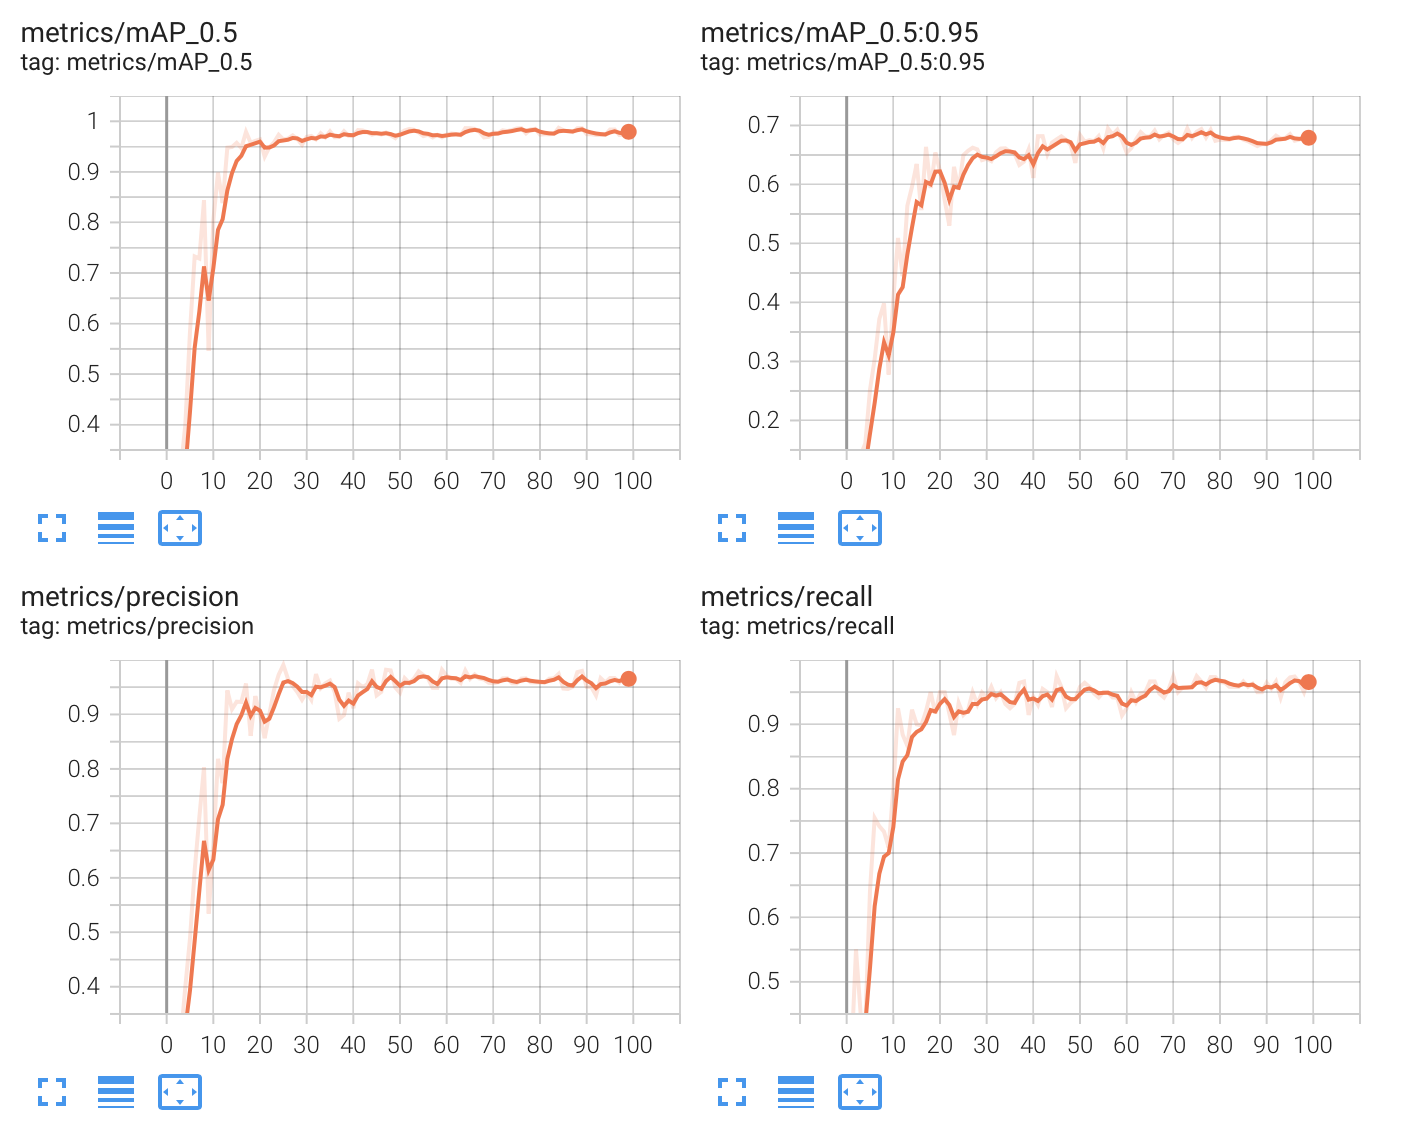
\includegraphics[width=12cm]{figs/metricas}
  \end{center}
\caption{Métricas del modelo entrenado para la detección de ratones.} \label{fig:metricas}
\end{figure}
\begin{figure}[h!]
  \begin{center}
    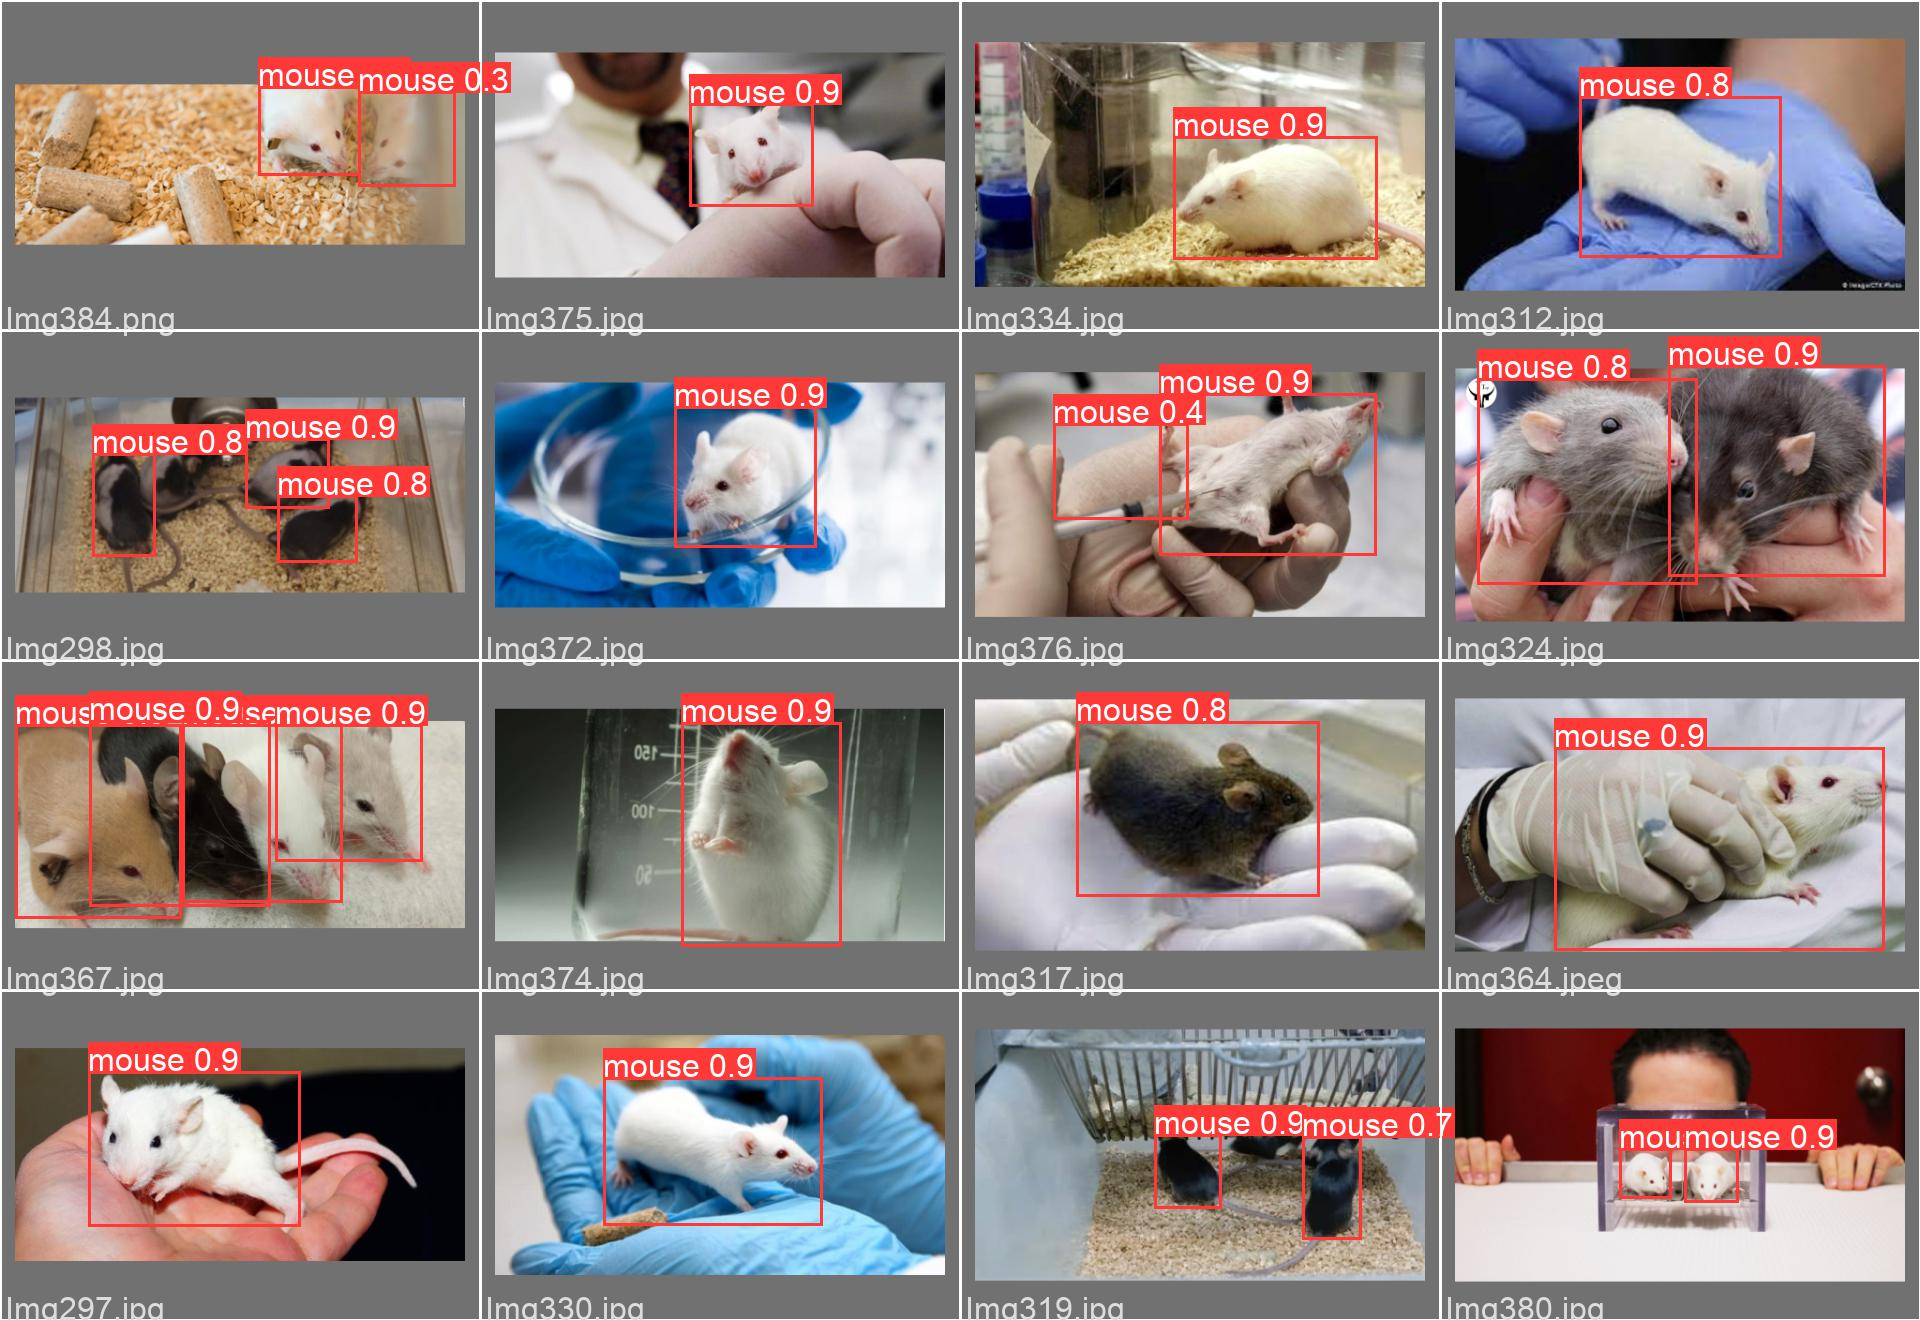
\includegraphics[width=12cm]{figs/precision}
  \end{center}
\caption{Detección de ratones con el modelo entrenado con YOLOv5.} \label{fig:precision}
\end{figure}
Finalmente, con el uso de Python y OpenCV, puede visualizarse la detección de ratones en tiempo real con la PiCamera y la Raspberry. 

A pesar de que se ha usado uno de los modelos más rápidos, en Raspberry el flujo de imágenes no es fluido. Debido a este motivo, la detección no es perfecta; pues hay detecciones incorrectas así como ocasiones en las que no detecta ratones (Figura \ref{fig:detec}).
\begin{figure}[h!]
  \begin{center}
    \subfigure[Detección correcta]{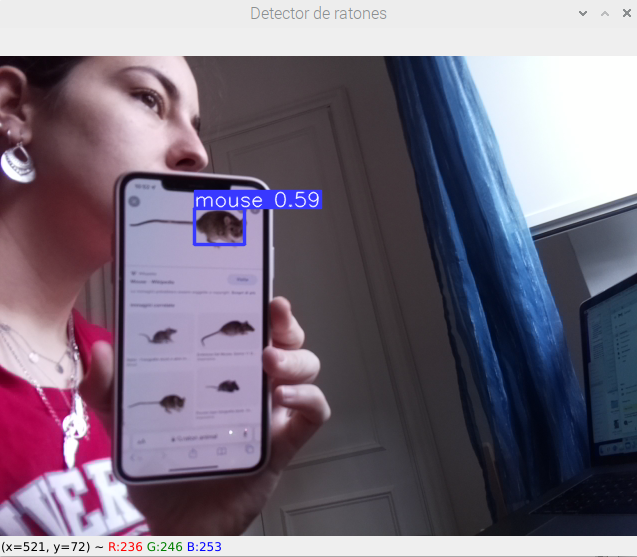
\includegraphics[width=7cm]{figs/correcta}}\hspace{1mm}
    \subfigure[Detección incorrecta]{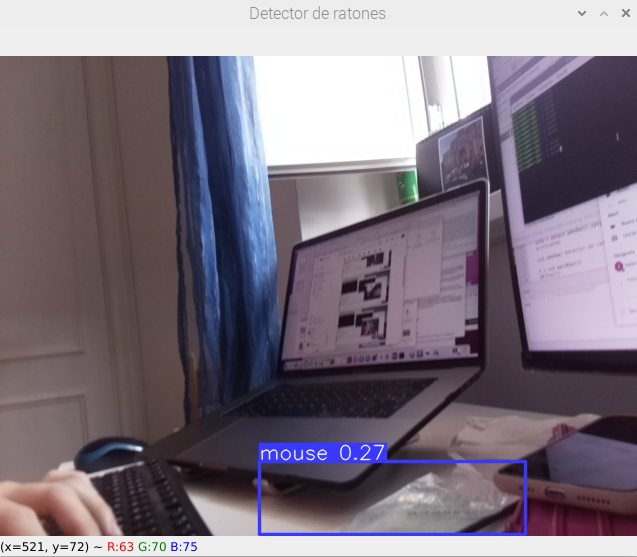
\includegraphics[width=7cm]{figs/incorrecta}}\hspace{1mm}
    \subfigure[No detección incorrecta]{\includegraphics[width=7cm]{figs/nodeteccion}}\hspace{1mm}
    \subfigure[No detección correcta]{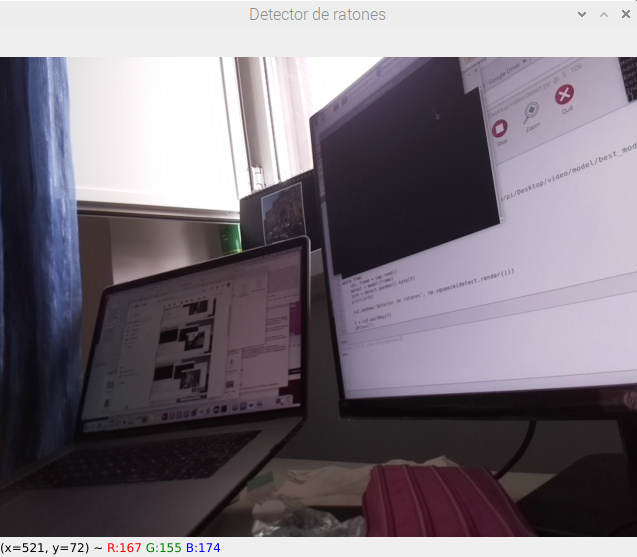
\includegraphics[width=7cm]{figs/nodeteccbien}}
  \end{center}
\caption{Detección de ratones con el modelo entrenado.} \label{fig:detec}
\end{figure}
